\documentclass[10pt]{article}
\usepackage[a4paper,margin=1in]{geometry}
\usepackage{amsmath,amssymb,amsthm}
\usepackage{booktabs}
\usepackage{graphicx}
\usepackage{microtype}
\usepackage[numbers,sort&compress]{natbib}
\usepackage{xcolor}
\usepackage[colorlinks=true,linkcolor=blue!50!black,citecolor=blue!50!black,urlcolor=blue!50!black]{hyperref}
\usepackage{array}
% Captions one step below body size, bold "Figure N:" label, so caption text
% is immediately distinguishable from running text. (Loaded after hyperref,
% as the caption package requires.)
\usepackage[font=small,labelfont=bf,skip=6pt]{caption}

% HARD RULE: no fabricated references. Every refs.bib entry was
% identity-verified against a primary source; as of 2026-07-17 no pending
% \citeph placeholders remain (the macro is retired).

\newcommand{\CFG}{\mathrm{CERT\_FG}}
\newcommand{\CBG}{\mathrm{CERT\_BG}}
\newcommand{\POSS}{\mathrm{POSSIBLE}}
\newcommand{\eps}{\varepsilon}
\newtheorem{proposition}{Proposition}
\newtheorem{lemma}{Lemma}

% Long unbreakable technical atoms (CERT_FG, H_1(...), file names) can
% otherwise push past the right margin; let TeX stretch interword space a
% little further before it resorts to an overfull line.
\emergencystretch=3em
% Ragged-right fixed-width column: in narrow table columns, justification
% cannot break words like "AdaptiveCertify" and overflows instead.
\newcolumntype{L}[1]{>{\raggedright\arraybackslash}p{#1}}

\title{INTACT: Sound Worst-Case Topological Certificates\\for Segmentation
Score Maps\thanks{Code, data and pre-registration record:
\url{https://github.com/arperon-labs/INTACT}}}
\author{Radoslav Loveck\'y\\Arperon\\[2pt]
{\small\texttt{info@arperon.com}}}
\date{Preprint v1}

\begin{document}
\maketitle

\begin{figure}[!ht]
\centering
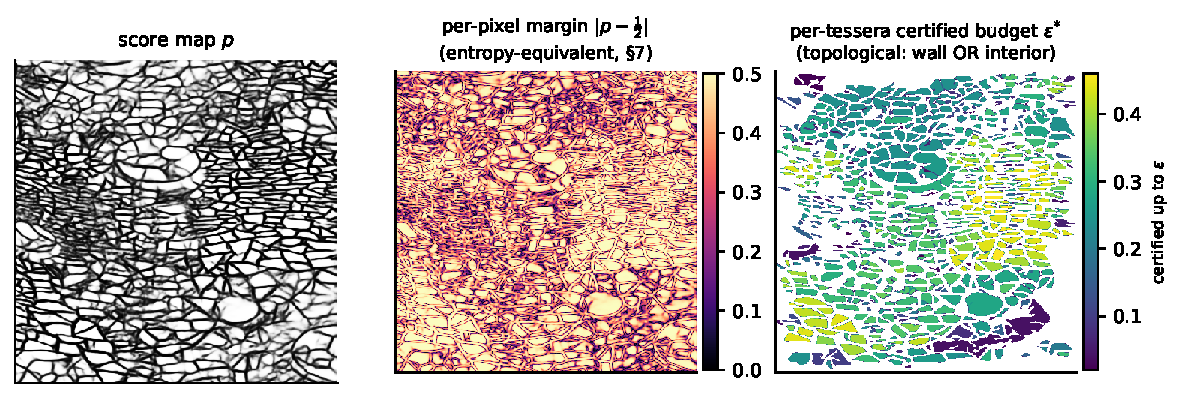
\includegraphics[width=\linewidth]{figs/fig_graded.pdf}
\caption{\textbf{The certificate is not a confidence map.} Left: a frozen
score map $p$ on a real mosaic crop. Middle: the per-pixel margin
$|p-\tfrac12|$ --- a monotone transform of predictive entropy
(\S\ref{sec:limitations}), which calls almost every pixel confident. Right:
what INTACT actually certifies --- each enclosed tessera painted by
$\eps^{*}$, the largest $\ell_\infty$ budget at which it \emph{provably}
remains an unfillable hole. The budgets are \emph{graded}: some tesserae
survive to $\eps{\approx}0.45$, others are lost by $\eps{\approx}0.05$,
because a hole dies when its \emph{wall} erodes as readily as when its
interior does --- a topological fact that no per-pixel confidence map
contains. Read off the exactly-nested sweep (\S\ref{sec:nesting}), on a
finer $\eps$ grid than Table~\ref{tab:real}; the crop is the one whose
certified-cycle count is closest to the 30-crop cohort mean.}
\label{fig:graded}
\end{figure}

\begin{abstract}
Consumers of segmentation rarely ask about pixel accuracy; they ask
topological questions --- how many connected structures are there, does
this line stay unbroken, how many enclosed regions does it bound.
Topology-aware training methods (the clDice and Betti-matching lineage)
improve such properties on average but guarantee nothing about any
particular output. We present INTACT (INference-Time Adversarial
Certificates for Topology): sound, worst-case topological certificates
for thresholded segmentation score maps. An $\ell_\infty$ uncertainty
band of radius $\eps$ around a frozen score map $p$ determines ---
exactly --- a lattice interval of reachable binary masks, between the certainly-foreground core
$\CFG=\{p-\eps>\tfrac12\}$ and the complement of the certainly-background
core $\CBG=\{p+\eps\le\tfrac12\}$. Over this interval we prove a two-mask
certification principle: a finite conjunction of monotone predicates
holds on every reachable mask iff it holds at the interval's two extremes
--- and both extremes are individually necessary, a minimal check that no
fixed budget of random sampling can replace. Instantiating the principle
yields five certified quantities --- certainly-foreground coverage,
certified connected components, certified enclosed regions (tesserae), a
strict certified-connectivity fraction, and certified 1-cycles --- holes
whose wall is certainly foreground and whose interior is certainly
background, so no in-budget perturbation can fill or breach them --- each
stated with its worst-case adversary and its scope caveat. The certificate
operates on perturbations of the score map; it is \textbf{not} an
end-to-end input-space certificate (composition with input-space methods
is an interface we state, not a result we claim).

The instantiation is not mechanical: our first cycle certificate,
$\beta_1$ of the certified foreground, was genuinely unsound ($H_1$ is not
monotone under foreground growth), and we report the counterexample, the
catch, and the fix as a section of the method, not a footnote. A
worst-case-exhaustive soundness harness attacks all four class-valued quantities --- coverage,
which is a pixel fraction with no per-instance support --- at the two
deterministic
extremes; on real model outputs it reports \textbf{0 violations in
16{,}675{,}936 checks}. On 30 real mosaic crops through a
frozen zero-shot grout-segmentation model the certificate is non-vacuous:
at $\eps=0.10$, 94\% of predicted grout length is certainly-foreground; at
the calibration-defined $\eps=0.40$, 60\%. Coverage, however, is not
connectivity --- the strict certified-connected fraction is always
smaller: 0.766 at $\eps=0.10$ and 0.343 at $\eps=0.40$, a modest
1.2--1.7$\times$ gap on real outputs (the order-of-magnitude gap appears
only on the near-tautological toy track, where the blurred maps fragment).
We report the two numbers separately rather than blur them into one.
\end{abstract}

\section{Introduction}\label{sec:intro}

A segmentation map is usually consumed through its topology. A radiologist
asks whether a vessel is interrupted; a conservator asks whether a mosaic's
grout network still separates every tile from its neighbours; an inspector
asks whether a crack
network is one connected system or several. Pixelwise scores answer none
of these questions directly, and a model that is 99\% accurate per pixel
can still be topologically wrong everywhere it matters.

A substantial literature addresses this at \emph{training time}:
topology-aware losses and metrics --- clDice for tubular structures
\citep{shit2021cldice}, persistent-homology losses
\citep{hu2019topo,clough2020topological}, Betti matching
\citep{stucki2023betti} --- shape the learned map so that its topology is
better \emph{on average}. What they do not provide is a guarantee about
any given output: after training, nothing tells the consumer which
components of \emph{this} prediction survive \emph{this} much uncertainty.

This paper takes the complementary, inference-time view. Given a frozen
score map $p$ and an $\ell_\infty$ budget $\eps$ on perturbations of $p$,
we compute topological statements that \textbf{hold on every mask
reachable within the budget},
and we prove and then \emph{test} that claim adversarially. The name is
the guarantee: INTACT certifies what remains \emph{intact} --- which
components stay connected, which lines stay unbroken, which holes stay
unfillable --- under any in-budget perturbation. The conceptual
ancestor is fifty years old: Benson's algorithm for unconditional life in
the game of Go \citep{benson1976} certifies a group alive under \emph{any}
sequence of opponent moves via a monotone fixpoint --- an adversarial
certificate, not a statistical one. Our certificate is the same move for
segmentation topology: a monotone construction (thresholding an
interval-bounded map) whose conclusions hold against the entire
perturbation band.

Contributions, each with its qualifier:
\begin{enumerate}
\item \textbf{The sandwich is exact} (\S\ref{sec:setting}).
  $\CFG$/\allowbreak$\POSS$/\allowbreak$\CBG$ partitions the image so
  that the reachable set of binary masks under any
  $\ell_\infty$-$\eps$ perturbation is \emph{exactly}
  \[
    \{M : \CFG \subseteq M \subseteq \lnot\CBG\}
  \]
  (Proposition~\ref{prop:sandwich}) --- thresholding is monotone and
  interval propagation through it is endpoint-exact, so the abstraction
  loses nothing.

\item \textbf{Two masks suffice, and both are needed}
  (\S\ref{sec:soundness}). Over that interval a
  finite conjunction of monotone predicates is certified by checking
  exactly the two extreme masks (Lemma~\ref{lem:extremes}); each extreme
  is individually necessary, and no fixed budget of random masks
  substitutes for either --- the image-topology instance of a classical
  three-valued duality (\S\ref{sec:related}), made exact and tight.
\item \textbf{Five certified quantities, each with adversary and caveat}
  (\S\ref{sec:quantities}): certainly-foreground coverage; certified
  $\beta_0$ components; certified enclosed tesserae; a strict
  certified-connectivity fraction; and certified 1-cycles as
  \emph{unfillable holes}, reported as the count of enclosed
  guaranteed-background regions and cross-checked against the rank of the
  image $H_1(\CFG\hookrightarrow\lnot\CBG)$ --- two related quantities that
  are not equal in general (\S\ref{sec:cycles}). We
  keep coverage and connectivity as two separate reported numbers, because
  they are different quantities --- a modest 1.2--1.7$\times$ apart on real
  outputs, an order of magnitude only on the near-tautological toy track
  (\S\ref{sec:covconn}).
\item \textbf{Adversarial self-verification as part of the method}
  (\S\ref{sec:correction}). A soundness harness exercises every certified
  class at the deterministic worst-case extremes of the reachable set
  (plus random reachable masks) and must also catch deliberately planted
  unsound certificates. An adversarial-verification
  pass over the registered claims caught a real unsoundness that the
  harness, as then configured, had missed --- our originally registered
  cycle certificate, $\beta_1(\CFG)$, is \emph{false} as a robustness
  claim --- before any real-model number was reported. We present the
  counterexample, why the original check missed it, and the corrected
  certificate.
\item \textbf{Non-vacuity on real model outputs} (\S\ref{sec:experiments}).
  On 30 real mosaic crops through a frozen zero-shot grout segmenter, the
  certificate holds with 0 violations in 16{,}675{,}936 checks and is far
  from empty: 94\% of predicted grout length is certainly-foreground at
  $\eps=0.10$, and 60\% survives even at the calibration-defined budget
  $\eps=0.40$, with dozens of certified components and hundreds of
  certified enclosed tesserae; the strict certified-connectivity fraction,
  now measured on real $p$, is 0.766 and 0.343 at those two budgets.
\end{enumerate}

\paragraph{Threat-model statement (read first).} The certificate as built
operates on perturbations of the \emph{score map} $p$: the adversary may
replace $p$ by any $p'$ with $\|p'-p\|_\infty \le \eps$. It is
\textbf{not} an end-to-end input-space certificate --- nothing here bounds
how far $p$ can move when the \emph{input image} is perturbed. The two
compose cleanly in principle: any input-space method that yields per-pixel
bounds on the score map (randomized smoothing
\citep{cohen2019smoothing,fischer2021segcert}, interval bound propagation
\citep{gowal2018ibp}) supplies exactly the interval field our machinery
consumes. We state this as an interface in \S\ref{sec:future}; we have not
built it, and no claim in this paper depends on it.

\paragraph{Domain.} Our primary testbed is GROUT \citep{lovecky2026grout},
a zero-shot (synthetic-only trained) EfficientNet-B3 U-Net segmentation
model for the grout lines of stone mosaics; the enclosed tiles are
\emph{tesserae}.
Nothing in \S\S\ref{sec:setting}--\ref{sec:correction} is specific to
mosaics --- the machinery consumes any soft map thresholded at $\tfrac12$
--- and we exercise that generality off-domain in \S\ref{sec:crossdomain}
with a cross-domain stress-test on two retinal-vessel datasets (DRIVE
\citep{staal2004drive} and CHASE\_DB1 \citep{fraz2012chase}, model-free
Frangi maps), where the soundness harness holds across a second modality.
The \emph{headline non-vacuity} numbers, however, are about the single
mosaic task and one frozen checkpoint, and we say so wherever it matters.

\section{Setting and threat model}\label{sec:setting}

\begin{figure}[t]
\centering
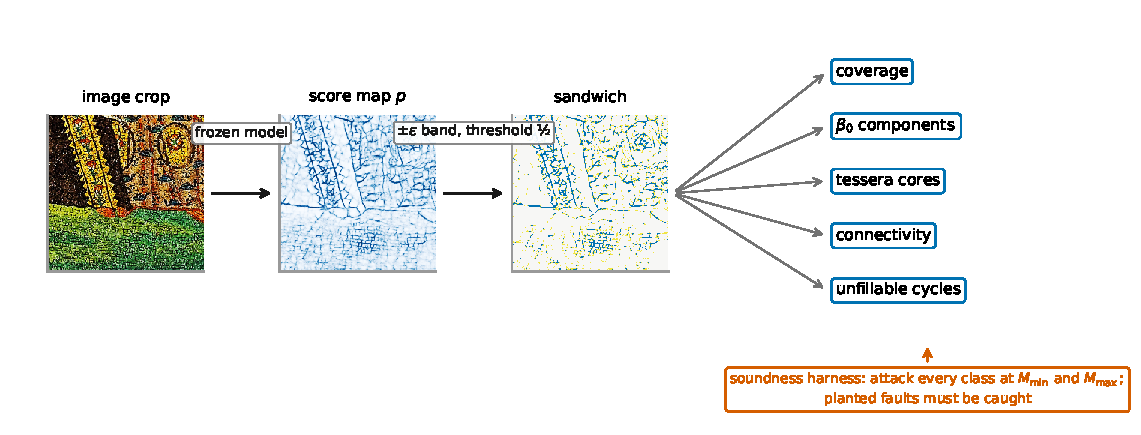
\includegraphics[width=\linewidth]{figs/fig_pipeline.pdf}
\caption{The INTACT pipeline. A frozen segmenter produces the score map
$p$; the $\pm\eps$ band thresholded at $\tfrac12$ induces the sandwich
($\CFG$ / $\POSS$ / $\CBG$); five certified quantities are read off, four of
which (components, tessera cores, cycles, connectivity segments) carry a
support the soundness harness attacks at the two adversarial extremes
$M_{\min}, M_{\max}$ (coverage is sound by $\CFG$-containment, not attacked),
with planted-fault regressions required to ring.}
\label{fig:pipeline}
\end{figure}

Let $p \in [0,1]^{H\times W}$ be a frozen score map (``grout
probability'' per pixel), binarised at threshold $\tfrac12$: the predicted
foreground is $\{p > \tfrac12\}$ (pipeline overview:
Figure~\ref{fig:pipeline}). The adversary picks any $p'$ with
$\|p'-p\|_\infty \le \eps$ and the consumer sees the mask
$M(p') = \{p' > \tfrac12\}$.

\paragraph{The sandwich.}
\begin{align*}
\CFG  &= \{\,x : p(x)-\eps > \tfrac12\,\} \quad\text{(certainly foreground)}\\
\CBG  &= \{\,x : p(x)+\eps \le \tfrac12\,\} \quad\text{(certainly background)}\\
\POSS &= \text{the complement} \quad\text{(the adversary's territory)}
\end{align*}
The asymmetry between the two tests is forced by the strict threshold rule
$M=\{p' > \tfrac12\}$, and is not a blemish: a pixel is certainly
foreground iff its lower endpoint clears the threshold strictly, and
certainly background iff its upper endpoint fails to --- which is the
\emph{non-strict} $p+\eps \le \tfrac12$. With a strict test on the
background side, a pixel at the exact tie $p+\eps=\tfrac12$ would be
called $\POSS$ despite being unable to cross the threshold, and the
proposition below would hold only up to such ties.

\begin{proposition}[reachable set, exact]\label{prop:sandwich}
$\{\,M(p') : \|p'-p\|_\infty \le \eps\,\}
 = \{\,M : \CFG \subseteq M \subseteq \lnot\CBG\,\}$.
\end{proposition}
\begin{proof}
($\subseteq$) For any admissible $p'$ and any $x \in \CFG$,
$p'(x) \ge p(x)-\eps > \tfrac12$, so $x \in M(p')$; symmetrically no
$x \in \CBG$ enters $M(p')$. ($\supseteq$) Given any $M$ with
$\CFG \subseteq M \subseteq \lnot\CBG$, set
$p'(x)=\min(p(x)+\eps,\,1)$ where $x \in M$ and
$p'(x)=\max(p(x)-\eps,\,0)$ otherwise. Then $p'$ is admissible, and
exactly two implications are needed: if $x \in M$ then $x \notin \CBG$,
so $p(x)+\eps > \tfrac12$ and hence $p'(x) > \tfrac12$; if
$x \notin M$ then $x \notin \CFG$, so $p(x)-\eps \le \tfrac12$ and
hence $p'(x) \le \tfrac12$. Therefore $M(p')=M$.
\end{proof}

\paragraph{Floating point.} In the implementation the interval
$[p-\eps,\,p+\eps]$ is widened outward by one ulp per endpoint
(\texttt{np.nextafter}; enabled by default) before the
comparisons, so rounding can only \emph{shrink} the certified sets, never
grow them. One consequence: an exact tie $p+\eps=\tfrac12$ has its
endpoint widened above $\tfrac12$ and is recorded as $\POSS$ rather than
$\CBG$. The computed sets are therefore the exact sets of
Proposition~\ref{prop:sandwich} minus a measure-zero tie set, always in
the direction of abstention --- the behaviour a safety-critical consumer
needs, since a pixel the budget could push either way is treated as
uncertain rather than silently certified.

Thresholding is a monotone operation and interval propagation through it
is endpoint-exact: the propagated interval is attained, which is what
Proposition~\ref{prop:sandwich} states set-theoretically. In abstract-interpretation terms
\citep{cousot1977}: the interval abstraction of the threshold operator is
\emph{exact} here, not merely sound.

Everything certified below is a statement quantified over the reachable
set of Proposition~\ref{prop:sandwich} --- equivalently, over every
admissible perturbation.

\paragraph{Structured adversaries.} Any perturbation class contained in
the $\ell_\infty$ ball inherits soundness by containment: every
certificate holds a fortiori against smooth fields, low-frequency noise,
or any other structured subset of the ball. What is surrendered is
exactness --- the reachable set of a structured class is generally not a
lattice interval, so Proposition~\ref{prop:sandwich}'s equality becomes
containment and the two-extreme check certifies against a superset of
what is strictly reachable: sound but conservative, with the conservatism
concentrated at $\POSS$ features smaller than the adversary's correlation
length. The tightness measure argument of \S\ref{sec:soundness} says why
this direction is the right one to be conservative in: correlated noise
makes coordinated $c$-pixel flips \emph{likely} rather than measure
$2^{-c}$, so a structured adversary is more dangerous per unit budget,
never less. Exact certification under structured classes is open
(\S\ref{sec:future}).

\paragraph{Where $\eps$ comes from.} So that $\eps$ is not an invented
number, the ``useful'' budget is calibration-defined: the median of the
confidence margin $|p-\tfrac12|$ over uncertain pixels
($0<\text{margin}<\tfrac12$), per map, median across maps, snapped to the
\emph{nearest} point of the swept grid. On the real track this gives $0.425 \to \eps=0.40$; the sweep
is $\eps \in \{0.02, 0.05, 0.10, 0.15, 0.25, 0.40\}$. Snapping to the
nearest point can move $\eps$ down, which weakens the adversary and so
makes certificates easier --- the one step in the pipeline that does not
err toward abstention. It is guarded by the split-half stability of the
estimator (\S\ref{sec:epsstab}), which selects the same grid point in 200
of 200 resamples, and by the exactly-nested sweep (\S\ref{sec:nesting}),
which shows what any mis-estimate would cost.

\paragraph{Conventions (part of the certificate's definition, not post-hoc
filters).}
Certificates take a region-of-interest mask and a physical scale floor.
The ROI is the whole frame on the mosaic tracks --- so the abstain
denominator there is the whole image --- and, on the retinal tracks, the
dataset's field-of-view mask eroded by six binary-erosion iterations. The
floor is a \emph{local-thickness} test rather than an area or diameter
test: a component survives iff it is non-empty after a morphological
opening with an elliptical structuring element of radius
$\max(1, \operatorname{round}(\text{floor}/2))$\,px, i.e.\ iff it
contains an inscribed disc of that radius. On the mosaic tracks the floor
is half the tessera-width scale, tessera width being the square root of the
median area of the 4-connected background components of the
$\eps$-\emph{independent} prediction $\{p > \tfrac12\}$ (components of
area $\ge 9$\,px; fallback width $6.0$\,px, hence a $3.0$\,px floor); on
the retinal tracks it is a fixed $1.0$\,px, since vessel calibre rather
than tessera size sets the scale. Foreground uses 8-connectivity,
background 4-connectivity (the standard dual pairing, so that curves
separate). All metrics are reported as
absolute counts alongside any fraction; ratios never stand alone. The
proofs are per-pixel or lattice-theoretic throughout, so
Proposition~\ref{prop:sandwich} and the coverage, component,
tessera-core and per-segment connectivity certificates carry to a cubical
grid of any dimension, with dimension entering only through the choice of
dual adjacency pairing (in 3D, 26/6 or 18/6 rather than 8/4). The cycle
certificate is the one exception, and we flag it rather than gloss it:
its persistence form generalises degreewise --- the image-rank
construction applies to $H_k$ for any $k$ --- but its \emph{enclosure}
form does not. By Alexander duality, background components that cannot
reach the border realise $H_{d-1}$, which is $H_1$ only when $d=2$; in
three dimensions the same computation counts enclosed voids, and $H_1$
tunnels have no enclosure form at all
(\S\ref{sec:generality}, \S\ref{sec:future}).

\paragraph{What is \emph{not} claimed.} (i) Nothing about the
input$\to p$ pipeline (threat-model statement, \S\ref{sec:intro}).
(ii) Nothing about correctness of $p$ against ground truth: the
certificate concerns robustness of \emph{this map's} topology to $\eps$,
not whether that topology is right. (iii) Nothing about $\POSS$ pixels ---
they are reported as the abstain fraction. (iv) No
claim that ``the whole grout network certainly stays connected''; the
connectivity certificate is per-segment (\S\ref{sec:conn}).

\section{Certified quantities and their soundness}\label{sec:quantities}

Table~\ref{tab:quantities} itemises the five certified quantities. Each
row is a worst-case claim over the entire reachable set, and each carries
the caveat that bounds what it means. This table is the paper's claim
surface: nothing stronger is asserted anywhere.

\begin{table}[t]
\centering
\caption{The five certified quantities. Every claim is quantified over
every reachable mask (Proposition~\ref{prop:sandwich}).}
\label{tab:quantities}
\small
\setlength{\tabcolsep}{4pt}
\begin{tabular}{L{0.15\linewidth}L{0.26\linewidth}L{0.15\linewidth}L{0.28\linewidth}}
\toprule
\textbf{Quantity} & \textbf{Certified claim} & \textbf{Worst-case adversary} & \textbf{Caveat} \\
\midrule
1. Coverage (certainly-fg fraction of grout length) &
every $\CFG$ pixel is foreground in every reachable mask &
per-pixel $\ell_\infty$-$\eps$ &
a \textbf{coverage} statement, NOT connectivity; a covered line pinched
through $\POSS$ can still split; fraction + absolute length \\
\addlinespace
2. Certified $\beta_0$ components ($\CFG$, 8-conn) &
each is connected in every reachable mask &
any reachable mask (all are supersets) &
$\CFG$'s \emph{own} components (absolute count), not the prediction's \\
\addlinespace
3. Certified enclosed tesserae ($\CBG$, 4-conn, ROI + scale floor) &
each stays fully background in every reachable mask &
any reachable mask &
certifies a tessera \textbf{core}, not the whole tile \\
\addlinespace
4. Certified-connected grout fraction (segments entirely in $\CFG$) &
segment endpoints stay connected under any $\eps$-perturbation &
all $\POSS \to$ background &
strictly $\le$ coverage; one $\POSS$ pinch disqualifies; modest on real
outputs ($1.2$--$1.7\times$), order-of-magnitude on toy \\
\addlinespace
5. Certified 1-cycles, two ways: \textbf{enclosed regions} ($\CBG$ walled
by $\CFG$, ROI + floor; the headline) and the \textbf{image rank} of
$H_1$ (\S\ref{sec:cycles}) &
each enclosed region is an unfillable, unleakable hole in every reachable
mask; the rank also lower-bounds $\beta_1(M)$ for every reachable $M$ &
both deterministic extremes &
\textbf{not} equal in general (\S\ref{sec:cycles}): the rank is smaller
when one cavity holds several $\CBG$ components split by $\POSS$, larger
where enclosure applies its ROI/floor. Only the rank bounds $\beta_1$; only
enclosure localises \\
\bottomrule
\end{tabular}
\end{table}

\subsection{Coverage (certainly-foreground fraction)}
The fraction of the skeleton of the predicted foreground that lies in
$\CFG$. We report it alongside its absolute certified length in pixels,
so the fraction never stands alone (Table~\ref{tab:real} caption). Sound by
Proposition~\ref{prop:sandwich}. The point bears repeating
because it is the most tempting overclaim in this design space: high
coverage does \textbf{not} mean the structure stays connected
(\S\ref{sec:conn}, \S\ref{sec:covconn}).

\subsection{Certified $\beta_0$ components}
The connected components of $\CFG$ itself (8-connectivity). Every
reachable mask $M$ satisfies $\CFG \subseteq M$, and adding pixels never
disconnects an already-connected set, so each $\CFG$ component remains
connected --- as a set of foreground pixels --- in every $M$. The count is
absolute and refers to $\CFG$'s own components; it is \emph{not} the
number of components of the prediction $\{p>\tfrac12\}$ (at large $\eps$,
$\CFG$ fragments and this count \emph{rises} --- visible in
Table~\ref{tab:real} --- precisely because it counts certified fragments).
A scope note a careful reader will want: this is a certificate about the
\emph{named} components (each stays connected in every reachable mask),
not a lower bound on $\beta_0$ of every reachable mask --- two certified
components can merge through $\POSS$, which is exactly why the count
rises with $\eps$. The quantity that would bound distinct structures from
below --- the rank of the image $H_0(\CFG \to \lnot\CBG)$, the degree-0
analogue of \S\ref{sec:cycles}'s cycle certificate --- is well-defined in
the same filtration; we leave its registration as a certified quantity to
future work.

\subsection{Certified enclosed tesserae}
The connected components of $\CBG$ (4-connectivity), after ROI and scale
floor. Each lies in the background of every reachable mask. This certifies
the tessera \emph{core} --- the region that certainly remains background
--- not the full extent of the tile.

\subsection{Certified connectivity (the strict number)}\label{sec:conn}
Skeletonise the predicted foreground within the ROI by Zhang--Suen thinning
(\texttt{skimage.\allowbreak morphology.\allowbreak skeletonize}) --- the
thinning rule fixes the
node degrees and hence the segment decomposition, so it is part of the
certificate's definition --- and reduce it to a
segment graph: nodes are junctions (degree $\ge 3$) and endpoints (degree
1); edges are the junction-to-junction skeleton segments. A segment is
\textbf{certified-connected} iff \emph{every} pixel of it lies in $\CFG$;
then its endpoints remain connected under any admissible perturbation,
because the whole segment is present in every reachable mask. A single
$\POSS$ pixel on the segment disqualifies it --- that pixel is the
adversary's, and the worst-case mask (all $\POSS\to$background) cuts the
segment there.

We report the certified fraction of segments and of skeleton length (the
absolute segment and length companions are in the Table~\ref{tab:real}
caption). By
construction this is bounded above by coverage; that gap is measured, not
hidden --- modest on real $p$ (1.2--1.7$\times$) and dramatic only on the
toy track (\S\ref{sec:covconn}). We explicitly do not claim
network-level connectivity --- only the per-segment guarantee.

\subsection{Certified 1-cycles (unfillable holes) --- the corrected
certificate}\label{sec:cycles}
A cycle of the prediction is worth certifying only if the adversary can
neither \emph{fill} it (turn its interior to foreground) nor \emph{leak}
it (break its wall). The certified object is therefore an
\textbf{unfillable hole}: a connected region of $\CBG$ (guaranteed
background in every reachable mask) enclosed by $\CFG$ (guaranteed
foreground). Two related computations, which are \emph{not} equivalent in general:
\begin{itemize}
\item \textbf{Enclosure form:} $\CBG$ components not reachable from the
  image border through $\lnot\CFG$ (the can-be-background region); this
  form is ROI/scale-floor filtered and provides localisation.
\item \textbf{Persistence form:} the rank of the image
  $H_1(\CFG \hookrightarrow \lnot\CBG)$, computed by cubical persistent
  homology \citep{cohensteiner2009image} with the three-level filtration
  $\CFG=0$, $\POSS=1$, $\CBG=2$ (gudhi \citep{gudhi}; intervals with
  birth $<0.5$ and death $>1.5$).
\end{itemize}
The two forms count different things, and we separate them rather than
identify them. The enclosure form counts \emph{enclosed
guaranteed-background regions}; the persistence form counts the
\emph{rank} of an inclusion-induced map. They diverge whenever one
enclosed cavity contains several $\CBG$ components split by $\POSS$: a
$\CFG$ annulus whose interior holds two $\CBG$ squares separated by a
$\POSS$ channel gives enclosure 2 but image rank 1 ---
$\beta_1(\CFG)=1$ while $\beta_1(\lnot\CBG)=2$, and the annulus
generator maps to the \emph{sum} of the two blob classes. Only the
persistence rank lower-bounds $\beta_1(M)$ for every reachable $M$ (at
$M=\CFG$ the two squares merge into a single hole). The enclosure count
stays sound as a \emph{per-region} statement --- each region is
guaranteed background and unleakable in every reachable mask, which is
what the soundness harness verifies --- but it is not a Betti number and
must not be read as one. This is the degree-1 instance of the
named-features-versus-rank-bound distinction drawn for $\beta_0$ earlier
in this section.

The two counts agree \textbf{exactly} on the clean regression cases
(ring-over-$\POSS$ $\to 0$; ring-over-$\CBG$ $\to 1$; a $3\times 3$ grid
of enclosed cells $\to 9$; the planted unsound cycle $\to$ not certified)
--- we pre-registered this equivalence as a prediction before
the persistence code ran, and it holds wherever each enclosed cavity
contains a single $\CBG$ component. On noisy maps the two counts separate
in both directions --- persistence above enclosure where enclosure applies
its ROI and scale floor, enclosure above persistence where a $\POSS$
channel subdivides one cavity --- and \S\ref{sec:hc4} gives the measured
decomposition. Localisation stays with the enclosure form: persistence
gives a certified \emph{count}, not per-cycle generators.

This definition is the \emph{corrected} one. It is not what we first built
--- \S\ref{sec:correction} reports what we first built, why it was wrong,
and how it was caught.

\begin{figure}[t]
\centering
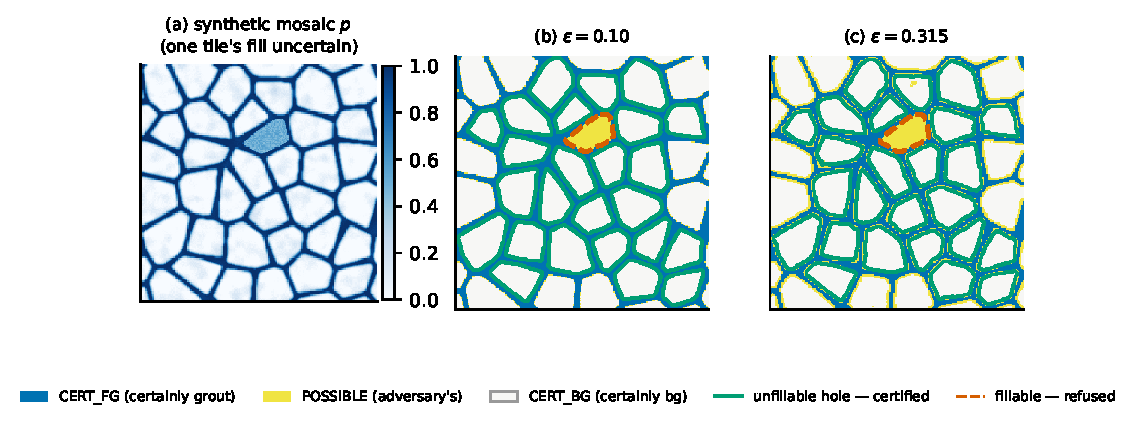
\includegraphics[width=\linewidth]{figs/fig_gallery.pdf}
\caption{The certified-cycle machine on a synthetic Voronoi mosaic (the
interactive companion's view, recreated for print). Confident tiles are
certified unfillable holes (green): $\CBG$ cores walled by $\CFG$. One
tile's interior is set model-uncertain to illustrate the distinction ---
its enclosed region holds no $\CBG$ core, so it is a fillable hole and is
\emph{refused} (dashed), exactly what the unsound $\beta_1(\CFG)$ of
\S\ref{sec:correction} would still have certified. (b)~$\eps=0.10$;
(c)~$\eps=0.315$ (off the swept grid, chosen to show the erosion): the thin
joints erode to $\POSS$ while the certified holes and the refusal both
persist.}
\label{fig:gallery}
\end{figure}

\subsection{Soundness: the structural argument and the adversarial
check}\label{sec:soundness}
Soundness has two layers, and we state the strength of each precisely.

\paragraph{The structural layer.} Each certificate is sound by
construction on top of Proposition~\ref{prop:sandwich}: $\CFG$ is
contained in the foreground of every reachable mask (quantities 1, 4);
connectivity is preserved under superset (quantity 2); $\CBG$ is contained
in the background of every reachable mask (quantity 3); and an unfillable
hole's wall and interior are pinned by both containments at once
(quantity 5). The outward one-ulp widening of \S\ref{sec:setting} only
shrinks CERT sets --- the safe
direction --- and the strict inequalities settle exact boundary ties
conservatively.

\paragraph{The adversarial layer.} An implementation can betray a proof,
so every certified class emitted by the pipeline is attacked by an
explicit soundness check: the \emph{deterministic worst-case extremes} of
the reachable set --- all $\POSS$ pixels to background (the minimal mask,
the worst case for anything foreground) and all $\POSS$ pixels to
foreground (the maximal mask, the worst case for anything background or
for filling a hole) --- plus random reachable masks. That the two
extremes suffice is not an empirical observation; it is a consequence of
the predicates' monotonicity:

\begin{lemma}[two extremes are exhaustive]\label{lem:extremes}
Write the reachable set as the lattice interval
\[
  \mathbb{I} = \{M : M_{\min} \subseteq M \subseteq M_{\max}\},
  \qquad M_{\min}=\CFG,\quad M_{\max}=\lnot\CBG
\]
(Proposition~\ref{prop:sandwich}). Call a predicate $\varphi(M)$
\emph{upward monotone} if $\varphi(M)$ and $M \subseteq M'$ imply
$\varphi(M')$, \emph{downward monotone} dually. Then a finite conjunction
of monotone predicates holds on all of $\mathbb{I}$ iff every
upward-monotone conjunct holds at $M_{\min}$ and every downward-monotone
conjunct holds at $M_{\max}$.
\end{lemma}
\begin{proof}
An upward-monotone conjunct that holds at $M_{\min}$ holds at every
$M \supseteq M_{\min}$; if it fails, $M_{\min} \in \mathbb{I}$ is itself
the witness. Dually at $M_{\max}$. A conjunction fails somewhere on
$\mathbb{I}$ iff some conjunct does.
\end{proof}

Each harness predicate is such a conjunction: a foreground class asserts
$S \subseteq M$ for its (already-connected) support --- upward monotone,
worst case $M_{\min}$; a background core asserts $S \cap M = \emptyset$
--- downward monotone, worst case $M_{\max}$; a cycle asserts its wall is
present (upward, $M_{\min}$) \emph{and} its interior stays background
(downward, $M_{\max}$) --- both extremes together; a connectivity segment
asserts a path exists --- path existence is upward monotone, worst case
$M_{\min}$. A violation counts as a broken certificate; a single one halts
the run before any headline number is emitted.

\paragraph{Tightness (both extremes necessary).}
Lemma~\ref{lem:extremes} makes the pair \emph{sufficient}; the certified
classes make each extreme \emph{individually necessary}
(Figure~\ref{fig:tightness}). Drop $M_{\max}$
and Figure~\ref{fig:counterexample}'s fillable ring is falsely certified
--- its cycle holds at $M_{\min}$ (wall present, interior open) yet is
filled at $M_{\max}$ once the $\POSS$ interior is forced to foreground
(\S\ref{sec:cycles}); drop $M_{\min}$ and Figure~\ref{fig:pinch}'s pinched
bar is falsely certified --- its segment spans at $M_{\max}$ yet is cut at
$M_{\min}$ once the $\POSS$ pinch is forced to background
(\S\ref{sec:conn}). By Lemma~\ref{lem:extremes} each failure localises at
exactly one extreme, never strictly interior; the foreground-support and
background-core classes only fix \emph{which} extreme is worst ($M_{\min}$
and $M_{\max}$ respectively, the direction in which the harness would
reject a support or core straying into $\POSS$), and a cycle forces both
at once. Since $M_{\min}$ is the worst case of every upward-monotone
conjunct and $M_{\max}$ of every downward one, neither extreme dominates
the other: neither can stand in for the other, and the check is \emph{minimal} at two
masks --- each extreme is itself a reachable mask on which the
dropped-extreme harness fails, so omitting either forfeits worst-case
certainty. Random sampling cannot restore it: by monotonicity $M_{\min}$
lies in \emph{every} non-empty upward-violation region and $M_{\max}$ in
every downward one, whereas a random draw detects a violation only by
landing in that region, of measure $2^{-c}$ in the number $c$ of $\POSS$
pixels that must turn adversarial in unison (an enclosure's whole
interior, a segment's separating cut). Taking $c$ large --- an enclosure
of growing area --- sends the per-draw detection $2^{-c}$ to zero, so for
any fixed budget $N$ the miss probability $(1-2^{-c})^{N}\to 1$; the two
extremes drive all $\POSS$ pixels at once and catch it with certainty. The
random reachable masks therefore add nothing to worst-case coverage; they
are retained only as a cross-check against implementation faults (an
independent review of the harness reached the same exhaustiveness
conclusion before Lemma~\ref{lem:extremes} was written down). The measure
argument is itself measured: a registered baseline
(Appendix~\ref{app:accounting}, Figure~\ref{fig:missrate}) plants fillable
rings and pinched bars with controlled in-unison count $c$, scores the
semantic events, and finds per-draw detection matching $2^{-c}$ exactly
under the uniform model --- polynomially better yet still vanishing under
the harness's own sampler --- with every planted violation caught at
exactly the predicted extreme and never the other.

\begin{figure}[t]
\centering
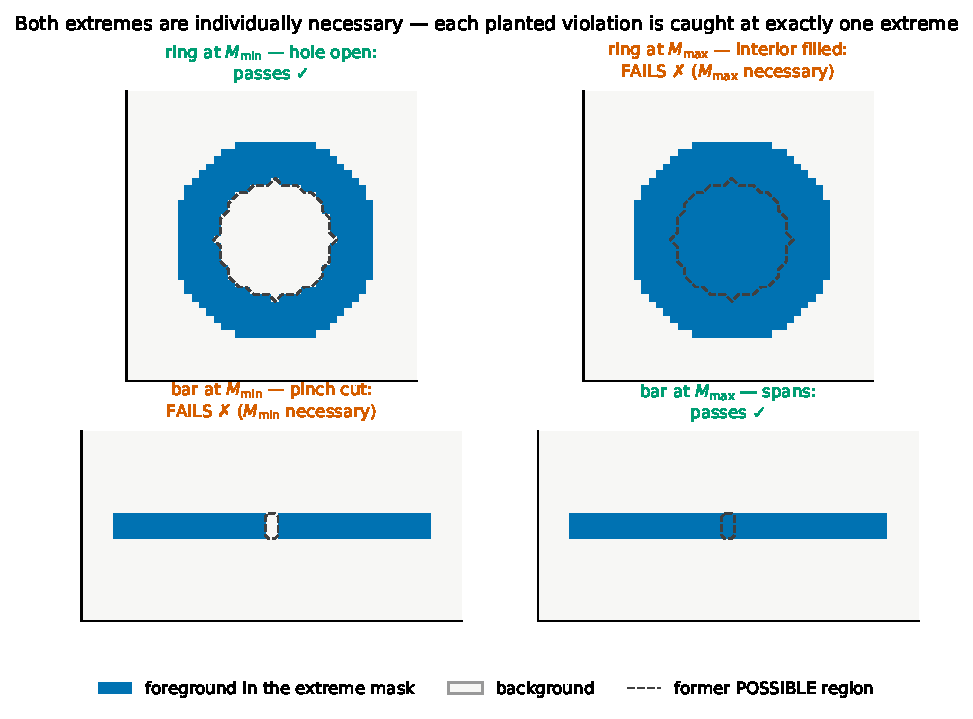
\includegraphics[width=0.9\linewidth]{figs/fig_tightness.pdf}
\caption{Tightness of the two-extreme check: the fillable ring's cycle
certificate holds at $M_{\min}$ (hole open) and fails only at $M_{\max}$
(interior filled), so dropping $M_{\max}$ falsely certifies it; the
pinched bar's segment spans at $M_{\max}$ and fails only at $M_{\min}$
(pinch cut), so dropping $M_{\min}$ falsely certifies it. Dashed outline:
the POSSIBLE region the adversary controls. By
Lemma~\ref{lem:extremes} each failure localises at exactly one extreme,
never strictly interior.}
\label{fig:tightness}
\end{figure}

The harness must also be able to \emph{fail}: deliberately planted unsound
certificates --- a foreground class intruding into $\POSS$, a background
core intruding into $\POSS$, a ``certified'' cycle over a fillable
interior, a ``certified-connected'' segment spanning a pinch --- are all
flagged by the same check (regression tests). A certificate system whose
alarm never rings is indistinguishable from one with no alarm; ours rings
on every planted fault. The one real fault (\S\ref{sec:correction}) was
caught not by this harness --- which did not yet know cycles were a class
--- but by an external adversarial-verification pass, after which the
harness was extended so that it would ring.

\paragraph{Result.} 0 violations for every certified class emitted on
each track and all swept $\eps$ --- all four classes (components, tessera
cores, corrected enclosure cycles, and connectivity segments) on both the
toy track and the real track
(16{,}675{,}936 checks over 30 crops).

\subsection{Generality of the construction}\label{sec:generality}

\paragraph{Interval fields (Proposition 1$'$).} Nothing in
Proposition~\ref{prop:sandwich} uses the uniformity of $\eps$: the proof
is per-pixel, so for any per-pixel interval field $[l(x), u(x)]$ on the
score map the reachable set of masks is exactly the lattice interval
between $\{l > \tfrac12\}$ and the complement of $\{u \le \tfrac12\}$, and
every certificate above applies unchanged to the resulting (non-uniform)
sandwich. Uniform $\eps$ is the corollary $l = p-\eps$, $u = p+\eps$, and
the composition interface of \S\ref{sec:future} is the corollary for
bounds supplied by input-space certification. The implementation is
already field-ready --- a per-pixel $\eps$ array broadcasts through the
identical code path (regression-tested) --- though the harness
results of \S\ref{sec:experiments} exercise only the uniform case.

\paragraph{The lattice form, and what else is monotone.} More
abstractly, the ingredients are an interval in a complete lattice and
monotone predicates: the sandwich is a three-valued (Kleene) abstraction
and the two-extreme check is the classical
optimistic/pessimistic-completion duality (\S\ref{sec:related}) --- we
claim the imaging instantiation, its exactness
(Proposition~\ref{prop:sandwich}), and its tightness
(\S\ref{sec:soundness}), not the lattice principle. The same two-mask
check therefore extends beyond topology: morphological erosion and
dilation are monotone lattice maps, so certified minimum thickness
(survival of erosion at $M_{\min}$), certified clearance (dually at
$M_{\max}$), and certified area intervals follow with no new theory ---
geometric certificates we flag but do not build here.

\paragraph{What is not monotone.} The recipe has a boundary, and
\S\ref{sec:correction}'s correction is its instance: perimeter, skeleton
length, convexity (which fails in both directions), curvature, and the
Euler characteristic are \emph{not} monotone under foreground growth ---
and $\beta_1$ fails directly, since growth fills holes, which is exactly why the naive
cycle certificate was unsound and the corrected one decomposes into a
wall conjunct (upward) and an interior conjunct (downward), one per
extreme. Non-monotone quantities require such a decomposition or a
different certificate; Lemma~\ref{lem:extremes} as stated does not cover
them, and we do not claim it does.

\section{The correction: an unsound cycle certificate, caught and
fixed}\label{sec:correction}

We consider this section part of the method. Adversarial
self-verification is not an afterthought to the certificate; it is what
makes the certificate credible --- a certificate system that cannot catch
a planted unsound certificate should not be trusted, and one that never
had to correct itself has probably not been attacked hard enough.

\subsection{What we originally certified}
As first registered, certified 1-cycles were computed as $\beta_1(\CFG)$,
with the justification: ``a loop in the minimal foreground persists in
all larger foregrounds.''

\subsection{The counterexample}
That justification is \textbf{false}: $H_1$ is not monotone under
foreground growth. Adding pixels can only merge or preserve components
(which is why quantity 2 \emph{is} sound), but it can \emph{destroy} holes
by filling them. Concretely (Figure~\ref{fig:counterexample}): let $\CFG$
be a ring whose interior is $\POSS$. Then $\beta_1(\CFG)=1$, and the
original certificate called this cycle robust. But the adversary may,
within budget, push every interior pixel above threshold --- a reachable
mask by Proposition~\ref{prop:sandwich} --- and the hole is gone:
$\beta_1(M)=0$. An in-budget perturbation destroys the ``certified''
cycle. The certificate was unsound. (In persistence terms the trap is
quantitative: this ring's superlevel bar has persistence $0.45$ ---
comfortably above $2\eps = 0.2$ --- yet the hole dies, because a long bar
need not straddle the threshold window at $\tfrac12$; see
\S\ref{sec:related}.)

\begin{figure}[t]
\centering
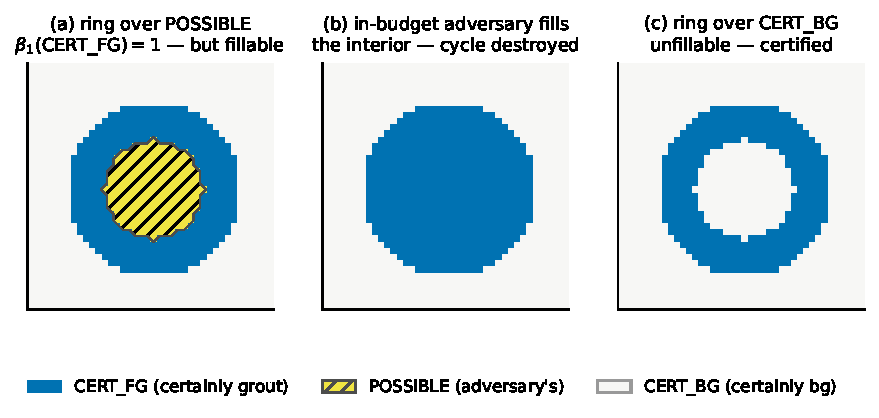
\includegraphics[width=\linewidth]{figs/fig_counterexample.pdf}
\caption{The $\beta_1$ counterexample (regression-test constructions,
$\eps=0.1$). (a) A $\CFG$ ring over a $\POSS$ interior:
$\beta_1(\CFG)=1$, but (b) the all-$\POSS\to$foreground extreme --- a
reachable mask --- fills the hole; certifying this cycle was unsound.
(c) The corrected certificate requires the interior to be $\CBG$: an
unfillable hole.}
\label{fig:counterexample}
\end{figure}

\subsection{Why the in-code check missed it}
The soundness harness of \S\ref{sec:soundness} existed at the time and
passed --- because it tested only the component and tessera classes.
Cycles were never attacked: the check enumerated worst-case masks for the
classes it knew about, and nobody had told it a cycle was a class. The
lesson is specific: \emph{every} certified predicate needs its own
adversary in the harness, and a predicate without one should be treated as
unverified.

\subsection{The fix}
The corrected certificate is the unfillable hole of \S\ref{sec:cycles}: a
cycle is certified iff its enclosed region is $\CBG$ (so it cannot be
filled) walled by $\CFG$ (so it cannot leak). The harness gained a
\texttt{cycle} class attacked at both extremes, and the regression suite
now encodes the exact counterexample: ring-over-$\POSS$ is \emph{not}
certified; ring-over-$\CBG$ is certified and survives the attack; a
planted unsound cycle is caught. The equivalence of the enclosure
computation with cubical image-persistence (\S\ref{sec:cycles}) was
pre-registered and checked afterwards as an independent cross-check on the
fixed definition; it held on the regression cases and was later refuted as
a general identity (\S\ref{sec:hc4}).

\subsection{Provenance}
The unsoundness was found on 2026-07-12 by an adversarial-verification
pass (two independent AI soundness reviewers attacking the registered
claims; the review record is preserved with the released code), \emph{before} the
real-model track ran: no real-$p$ number was ever reported under the
unsound definition. In the same pass, a metric-semantics overclaim was
corrected: a ``certified component fraction'' (predicted components
$\ge$50\%-covered by $\CFG$) was renamed to a coverage proxy, because a
$\ge$50\%-covered component pinched through $\POSS$ can still split ---
coverage is not connectivity, the recurring theme of this paper. The
registry preserves the original claims verbatim alongside the correction
addendum; the paper you are reading states only the corrected forms.

\section{Experiments}\label{sec:experiments}

\paragraph{Setup.} Real track (T-real): 30 real mosaic crops (the full
frozen evaluation set) through a frozen zero-shot GROUT
checkpoint (\texttt{grout\_b3\_zeroshot\_v1}) \citep{lovecky2026grout};
$p$ is the sigmoid of the model's patch logits. Crops are
$512\times512$\,px, the unit the runtimes of Appendix~\ref{app:compute}
are quoted per. Toy track (T-toy): 24 synthetic $256\times 256$
mosaic masks from our own generator with simulated scores
\[
  p=\mathrm{clip}\!\left(\mathrm{GaussianBlur}(\text{mask},\sigma{=}1.3)+
  \mathcal{N}(0,0.07^2)\right)
\]
--- retained strictly as a validation track
(\S\ref{sec:toy}). Sweep and conventions as in \S\ref{sec:setting}; seeds
fixed. Table~\ref{tab:toy} reports the toy run that carries the
persistence-cycle and connectivity columns. The
regression suite --- including the planted-unsound and counterexample
cases --- passes (\S\ref{sec:repro}).

\subsection{T-real: sound and non-vacuous on real model
outputs}\label{sec:real}

\begin{figure}[t]
\centering
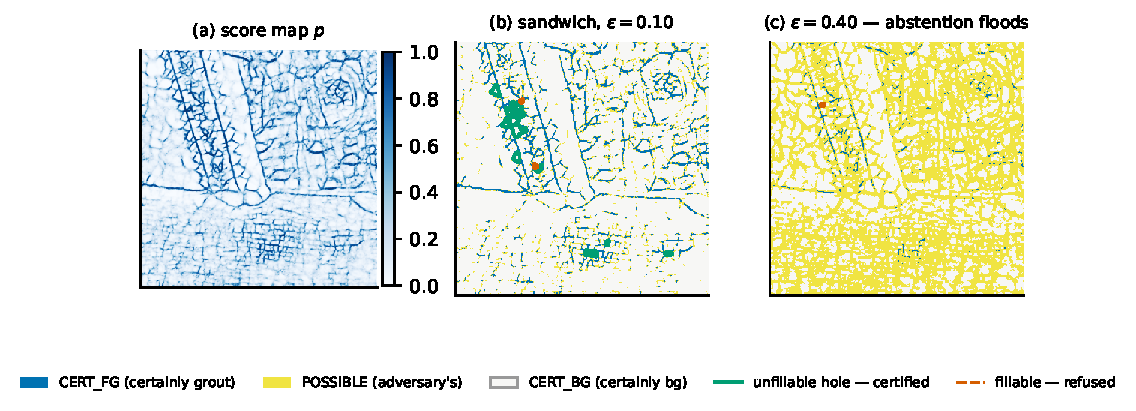
\includegraphics[width=\linewidth]{figs/fig_anatomy.pdf}
\caption{Anatomy of the certificate on a real crop --- the
\emph{worst-coverage} crop at $\eps=0.10$ by the registered metric
(\texttt{crop\_byzantine\_01}), not a curated example. (a) frozen-model
score map; (b) the sandwich at $\eps=0.10$ --- $\CFG$ grout (blue),
$\CBG$ tesserae (grey), $\POSS$ (yellow) --- with certified unfillable
holes outlined in green; (c) at the calibration-defined $\eps=0.40$ the
abstention band floods and fewer classes survive: certification degrades
monotonically (\S\ref{sec:nesting}), never silently.}
\label{fig:anatomy}
\end{figure}

Soundness first, because nothing else matters if it fails: the soundness
gate passes with \textbf{0 violations in 16{,}675{,}936 checks} across all
four certified classes this run emitted (components, tessera cores,
corrected cycles, and connectivity segments) and all
$\eps$ (\S\ref{sec:soundness}). The certificate then turns out to
be far from vacuous on real outputs (Table~\ref{tab:real},
Figure~\ref{fig:sweep} left).

\begin{table}[t]
\centering
\caption{T-real: certified quantities vs.\ $\varepsilon$ (frozen zero-shot model on 30 real $512\times512$ crops; per-crop means). No ratio stands alone: the denominators are $\eps$-independent --- coverage and conn-len over a mean skeleton length of $24{,}728.9$\,px per crop, conn-seg over $2{,}739.8$ segments, abstain over the ROI (here the whole crop). Numerators at $\eps=0.10/0.40$: certified length $23{,}408.1/14{,}969.8$\,px, certified segments $2{,}173.2/1{,}003.5$. Each fraction is the mean of the per-crop ratios, not the ratio of the means.}
\label{tab:real}
\small
\begin{tabular}{lrrrrrrrr}
\toprule
\textbf{eps} & \textbf{coverage} & \textbf{conn-len} & \textbf{conn-seg} & \textbf{\#comp} & \textbf{\#tess} & \textbf{\#cyc-encl} & \textbf{\#cyc-pers} & \textbf{abstain} \\
\midrule
0.02 & 0.988 & 0.921 & 0.916 & 17.9 & 530.5 & 471.5 & 740.6 & 0.016 \\
0.05 & 0.971 & 0.848 & 0.841 & 18.1 & 533.2 & 462.9 & 684.9 & 0.040 \\
0.10 & 0.942 & 0.766 & 0.761 & 20.3 & 537.3 & 439.0 & 606.6 & 0.080 \\
0.15 & 0.908 & 0.700 & 0.696 & 22.5 & 540.2 & 411.4 & 532.0 & 0.123 \\
0.25 & 0.823 & 0.577 & 0.575 & 30.2 & 536.4 & 342.7 & 398.4 & 0.219 \\
0.40 & 0.598 & 0.343 & 0.348 & 41.7 & 474.6 & 171.4 & 186.7 & 0.438 \\
\bottomrule
\end{tabular}
\end{table}


Readings. At an illustrative mid-sweep $\eps=0.10$, \textbf{94\%} of predicted grout
length is certainly-foreground with 20.3 certified components and
439.0 certified enclosed cycles per crop on average --- and, now measured
on real $p$, \textbf{0.766} of grout length is certified to stay
\emph{connected} (unbroken). The model is
confident on these crops, so the calibration-defined useful budget is
large (0.425, snapped to 0.40); even there \textbf{60\%} of grout length
is certainly-foreground and \textbf{0.343} is certified-connected, with
41.7 certified components and 171.4
certified cycles (per-crop means). Worst-case over the 30 crops --- the
right headline for a worst-case paper --- the cohort floors hold: coverage
0.187 and certified connectivity 0.028 at $\eps=0.40$ (each the minimum over
the 30 crops, on \emph{different} crops; Figure~\ref{fig:worstcrop},
Appendix~\ref{app:tables}, shows the full per-crop distribution). Our
pre-registered non-vacuity criterion --- at least 50\% of grout length
certainly-foreground, with at least one certified component, at the useful
$\eps$ --- passes; the pre-registered kill condition (under 10\% certified
at every useful $\eps$) is not triggered. The component count \emph{rises} with $\eps$
(17.9 $\to$ 41.7) --- that is $\CFG$ fragmenting, counted as
certified fragments, not evidence of more structure.

\begin{figure}[t]
\centering
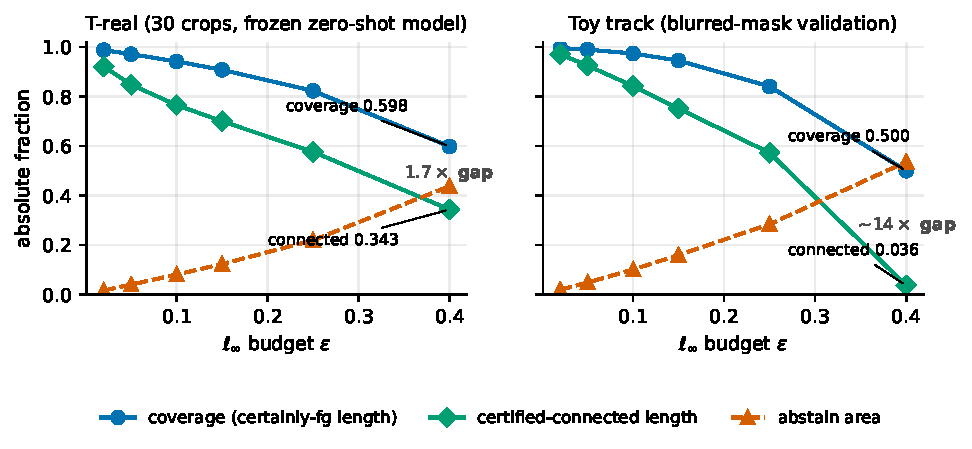
\includegraphics[width=\linewidth]{figs/fig_sweep.pdf}
\caption{Certified fractions vs.\ $\eps$, both tracks (coverage,
certified-connected length, abstain). Left (T-real, 30 crops): the
coverage-vs-connectivity gap is a \emph{modest} 1.7$\times$ at $\eps=0.40$
(0.598 vs 0.343) --- the confident model keeps most segments entirely
inside $\CFG$. Right (T-toy): the same gap collapses to ${\sim}14\times$
(0.500 vs 0.036), an artifact of the blurred toy maps whose skeletons
fragment \emph{en masse}. Same three series, same $y$-scale; the panels'
contrast is the point (\S\ref{sec:covconn}).}
\label{fig:sweep}
\end{figure}

\subsection{Coverage is not connectivity --- the headline
pair}\label{sec:covconn}

The largest number in this paper (94\% coverage) is a coverage statement.
The corresponding \emph{connectivity} certificate --- grout that certainly
stays unbroken --- is a different, strictly smaller number, and we report
both everywhere, never one for the other. We have now
measured it on real $p$: at the useful $\eps=0.40$, coverage is 0.598
while the strict certified-connected length fraction is \textbf{0.343} ---
a \textbf{1.7$\times$} gap (\textbf{1.2$\times$} at $\eps=0.10$). The gap
is real --- connectivity is always the smaller number --- but on
real model outputs it is \emph{modest}, because the confident model keeps
most segments entirely inside $\CFG$.

The order-of-magnitude gap lives only on the near-tautological toy track,
where at $\eps=0.40$ coverage is 0.500 versus certified-connected length
\textbf{0.036} (segment fraction 0.062) --- a \textbf{${\sim}14\times$}
collapse (Figure~\ref{fig:sweep} right; Figure~\ref{fig:pinch} shows the
mechanism). That collapse is a property of the toy maps, not the
certificate: the toy scores are lightly-blurred masks whose skeletons turn
POSSIBLE \emph{en masse} at large $\eps$, whereas the real maps are sharp
enough that connectivity largely survives (0.343 of grout length certified
unbroken even at the largest calibrated budget). Reporting the two numbers
separately still matters --- blurring them converts a sound coverage
statement into an unsound connectivity claim, the same failure mode as
\S\ref{sec:correction} at the level of prose rather than code --- but the
real-track headline is a 1.7$\times$ gap, not an order of magnitude.

\subsection{T-toy: validation track, with its caveat stated
verbatim}\label{sec:toy}

The toy scores are $\mathrm{GaussianBlur}(\text{GT mask},\sigma{=}1.3) +
\text{noise } 0.07$ --- in the words of the results file: ``a
lightly-blurred copy of the answer key. Certifying that its topology
survives small perturbations is close to tautological, and the `useful
$\eps$' is calibrated from the \emph{same} $p$, so clearing 50\% is partly
self-fulfilling. These numbers demonstrate the machinery runs and produces
non-empty certificates on plausible-looking input --- nothing about
real-model behavior.'' We still print the toy table because engineered maps
are where soundness is easiest to attack and where the persistence-cycle
(persistence cycles, connectivity) were first validated --- not because it
is the only track carrying them; the real track now does too
(Table~\ref{tab:real}, \S\ref{sec:real}).

\begin{table}[t]
\centering
\caption{Toy track (24 synthetic maps): all columns, including the certified-connected fractions and the persistence cycle counts. Toy $p$ is a blurred copy of the ground truth --- validation of the machinery, not evidence about real-model behaviour.}
\label{tab:toy}
\small
\begin{tabular}{lrrrrrrrr}
\toprule
\textbf{eps} & \textbf{coverage} & \textbf{conn-len} & \textbf{conn-seg} & \textbf{\#comp} & \textbf{\#tess} & \textbf{\#cyc-encl} & \textbf{\#cyc-pers} & \textbf{abstain} \\
\midrule
0.02 & 0.996 & 0.971 & 0.969 & 0.7 & 185.8 & 151.71 & 214.58 & 0.019 \\
0.05 & 0.990 & 0.925 & 0.926 & 0.6 & 180.4 & 146.38 & 203.08 & 0.048 \\
0.10 & 0.974 & 0.842 & 0.854 & 0.6 & 169.4 & 135.12 & 183.96 & 0.101 \\
0.15 & 0.945 & 0.752 & 0.773 & 0.8 & 157.0 & 117.67 & 152.04 & 0.159 \\
0.25 & 0.841 & 0.572 & 0.598 & 3.5 & 134.6 & 71.12 & 73.25 & 0.284 \\
0.40 & 0.500 & 0.036 & 0.062 & 18.1 & 28.2 & 0.04 & 1.38 & 0.536 \\
\bottomrule
\end{tabular}
\end{table}


On this run's own calibration ($0.361 \to \eps=0.40$) the
$\ge$50\%-coverage criterion narrowly fails (0.4998) --- reported for
completeness; per the caveat above, toy non-vacuity is illustrative either
way. Soundness on the toy track: 0 violations, including the connectivity
predicate.

\begin{figure}[t]
\centering
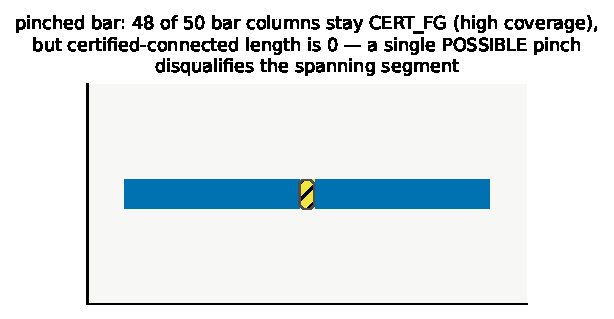
\includegraphics[width=0.6\linewidth]{figs/fig_pinch.pdf}
\caption{Why coverage $\ne$ connectivity (regression-test construction,
$\eps=0.1$): 48 of 50 bar columns stay $\CFG$ (high coverage), but the
two-pixel $\POSS$ pinch disqualifies the spanning segment ---
certified-connected length 0.}
\label{fig:pinch}
\end{figure}

\subsection{Nesting}\label{sec:nesting}
Certificates over decreasing $\eps$ are monotone-nested ---
$\CFG(\eps') \supseteq \CFG(\eps)$ for $\eps' \le \eps$, exact set
containment, so every certified quantity that is a \emph{measure} of the
certified sets --- coverage, certified length, abstain fraction --- is
monotone along the sweep. Counts are not, and the tables show it:
component and cavity counts are not monotone functionals of set inclusion
(\S\ref{sec:generality}), so \#comp and \#tess move non-monotonically in
Tables~\ref{tab:real} and \ref{tab:toy} as $\CFG$ fragments and $\CBG$
merges. One topological count \emph{is} provably monotone: by the diagram
identity of \S\ref{sec:hc4} the persistence-form cycle count at $\eps$ is
the number of points of $p$'s fixed superlevel diagram straddling
$[\tfrac12-\eps, \tfrac12+\eps]$, and widening $\eps$ can only shrink
that set, so \#cyc-pers is non-increasing in $\eps$ --- on every crop
individually, not merely in the mean. Exact set containment is asserted
and unit-tested (a pre-registered prediction; it holds on both tracks, and
registers the induced monotonicity of the coverage column). This is the hook for the graded extension of
\S\ref{sec:future}: the sandwich family over $\eps$ \emph{is} a nested
($\alpha$-graded) structure already.

\subsection{Persistence vs enclosure: a registered equivalence,
refuted}\label{sec:hc4}
We pre-registered the two computations of \S\ref{sec:cycles} as
equivalent. That is confirmed on the regression cases ($0/1/9$ on
ring-over-$\POSS$ / ring-over-$\CBG$ / $3\times 3$ grid of holes;
planted-unsound not certified) and \textbf{refuted as a general
identity} --- we record the refutation rather than quietly narrowing the
claim, as with \S\ref{sec:correction}. The two columns diverge in
\emph{both} directions, for two distinct reasons. Persistence exceeds
enclosure where enclosure applies the ROI and scale floor: on noisy toy
maps at $\eps=0.40$, persistence 1.38 vs floored enclosure 0.04 (per-map
means), the difference being sub-floor debris the definition excludes.
Enclosure exceeds persistence where a $\POSS$ channel subdivides one
cavity into several guaranteed-background regions
(\S\ref{sec:cycles}). On real $p$ this happens on 9 of the 30 crops at
$\eps=0.25$ and again at $\eps=0.40$ --- but never in the aggregate: the
cohort means in Table~\ref{tab:real} keep persistence above enclosure at
every budget, so the second direction is visible only per crop. The
equivalence therefore holds exactly when each enclosed cavity contains a
single $\CBG$ component, and not otherwise. The enclosure column remains
the headline count --- it is the localisable, per-region certificate ---
and the persistence column is reported alongside it as the rank bound,
not as the same number measured twice.

A second, different identity does hold, and was pre-registered before the
check ran: the persistence-form count
at \emph{every} swept $\eps$ equals the number of points of $p$'s own
superlevel diagram straddling the window $[\tfrac12-\eps, \tfrac12+\eps]$
--- verified exactly on every crop and every $\eps$
(a registered check; \S\ref{sec:repro}), so the entire $\eps$-sweep of certified
cycles is derivable from one diagram per crop, and \S\ref{sec:related}'s
rank identity is machine-checked rather than asserted.

\subsection{The $\eps$ estimator is split-half stable}\label{sec:epsstab}

Because $\eps$ is estimated (median confidence margin,
\S\ref{sec:setting}) rather than chosen, its stability is an empirical
question, and we register and measure it: across 200 random 15/15 splits
of the real crops, the calibration estimator's split-half drift is median
0.016 (maximum 0.071) --- small against the 0.15 gap between adjacent
sweep points at the operating budget --- and the two halves select the
\emph{same} grid point in 200 of 200 resamples, so the held-out certified
quantities are identical by construction. We do not \emph{learn} $\eps$
against the certified quantities, and would not: the band is the
assumption the certificate is conditioned on, and optimizing it against
certified counts would invert the semantics (a band chosen to flatter the
model certifies nothing about the domain). The estimator is
certificate-blind by design --- it reads only the score map's margins ---
and the exactly-nested sweep (\S\ref{sec:nesting}) already quantifies the
consequence of any mis-estimate.

\subsection{Cross-domain replication: two retinal-vessel
datasets}\label{sec:crossdomain}

Nothing in \S\S\ref{sec:setting}--\ref{sec:correction} is specific to
mosaics (\S\ref{sec:generality}), so we stress-test the certificate off the
mosaic domain entirely, on retinal blood-vessel maps --- the setting where
connectivity is the \emph{clinical} question. We use DRIVE
\citep{staal2004drive} (20 images) and CHASE\_DB1 \citep{fraz2012chase}
(20 images) and, with \textbf{no trained model}, build a score map $p$ per
image from multiscale Frangi vesselness \citep{frangi1998vessel} under
three monotone normalizations (cbrt, sqrt, log) with an Otsu-calibrated
logistic, then run the identical certificate.

\begin{figure}[t]
\centering
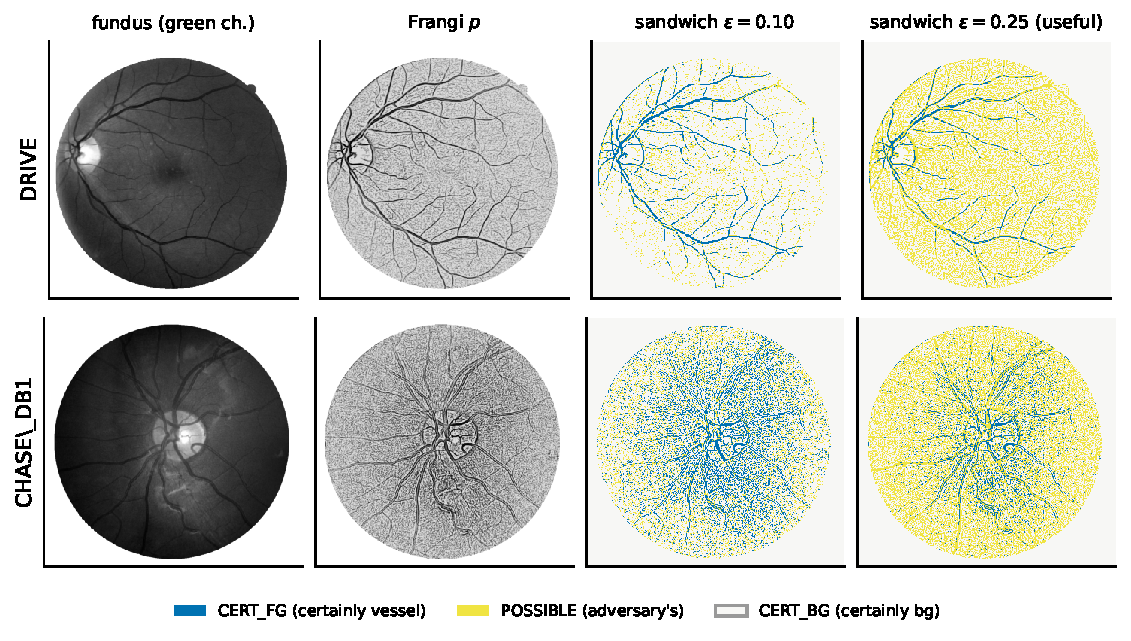
\includegraphics[width=\linewidth]{figs/fig_vessels.pdf}
\caption{The certificate on real retinal vessels (DRIVE and CHASE\_DB1),
model-free Frangi score maps, no training or checkpoint. Per row: fundus
green channel $\to$ Frangi $p$ $\to$ the $\pm\eps$ sandwich at a small budget
($\eps=0.10$, most of the vessel tree certified blue) and at the useful
budget ($\eps=0.25$, the certificate abstains --- yellow --- over
the thinner, noisier regions, more so on CHASE's over-segmented map). The
identical harness certifies both domains.}
\label{fig:vessels}
\end{figure}

\begin{figure}[t]
\centering
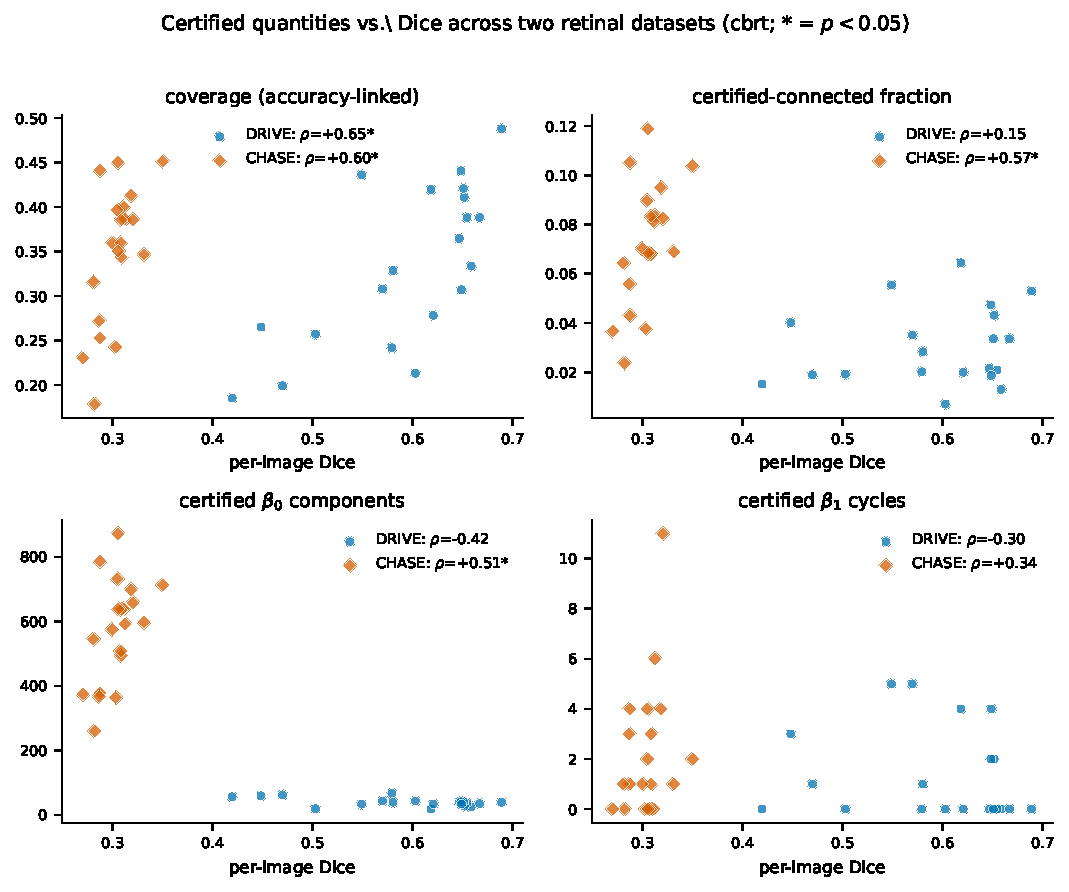
\includegraphics[width=\linewidth]{figs/fig_decoupling.pdf}
\caption{Per-image Dice vs.\ each certified quantity across DRIVE and
CHASE\_DB1 (primary cbrt normalisation; Spearman $\rho$ per dataset,
$*$~=~$p<0.05$). Coverage tracks Dice on both sets; the topological
invariants scatter on DRIVE but slope up on CHASE's degenerate,
over-segmented maps (Dice ${\approx}0.30$, $\beta_0$ counts in the
hundreds). Read the two clouds, not one trend line: the same quantity
correlates on one dataset and not the other.}
\label{fig:decoupling}
\end{figure}

\paragraph{Soundness holds cross-domain --- even on degenerate maps.} The
headline is negative space: across both datasets and all three
normalizations the soundness harness reports \textbf{0 violations in
10{,}578{,}388 checks} (DRIVE 2{,}963{,}152 at the full 16-mask setting;
CHASE 7{,}615{,}236 at 4 masks --- the two deterministic extremes plus two
cross-checks, exhaustive by Lemma~\ref{lem:extremes}, for the denser vessel
maps). This includes a genuinely adversarial regime for the certificate:
CHASE's cbrt normalization badly over-segments (median foreground
${\approx}29\%$ of the field of view, per-image Dice against the manual
tracing only 0.30; visible as the noisier map in
Figure~\ref{fig:vessels}), so the certificate must reason about
\emph{hundreds} of
certified components and thousands of connectivity segments per image ---
and it stays sound. A worst-case certificate that only held on well-behaved
maps would be far less useful; ours holds regardless of the underlying
prediction's quality.

\paragraph{Coverage is accuracy-linked; the topological certificates are
not simple Dice proxies} (Figure~\ref{fig:decoupling}). Correlating each
per-image certified quantity with that image's Dice (Spearman $\rho$,
primary cbrt normalization): coverage tracks Dice on both datasets
($\rho=+0.65$ on DRIVE, $+0.60$ on CHASE, both $p<0.05$) --- expected, since
coverage is essentially a confidence measure. The topological invariants
behave differently and \emph{inconsistently}: on DRIVE they
decouple from Dice (certified-connected fraction $\rho=+0.15$, $\beta_0$
$\rho=-0.42$, both n.s.), whereas on CHASE's degenerate cbrt maps they
correlate ($\rho=+0.57$, $+0.51$, both $p<0.05$) --- because in that
over-segmented regime more certified structure and less-bad accuracy
degrade together; under the better-behaved sqrt/log normalizations they
decouple on both datasets. The reading is not ``topology is
orthogonal to accuracy'': it is that the certified topological quantities
are \textbf{not reducible to Dice}, and their relationship to it is
regime-dependent --- so they must be reported as their own numbers (the
recurring theme of \S\ref{sec:covconn}), never inferred from an accuracy
score. The full per-transform $\rho$ table lives in the committed results
files.

\subsection{An inter-rater budget: $\eps$ from annotation
disagreement}\label{sec:interrater}

Where two human tracings exist, $\eps$ need not come from the model's own
margins (\S\ref{sec:setting}) --- it can be read from \emph{inter-observer
disagreement}, the irreducible uncertainty of the task itself. On the CHASE
images with two independent manual tracings, the median confidence margin
$|p-\tfrac12|$ over the pixels the two annotators label differently is
0.246, snapping to $\eps=0.25$ (the two tracings agree at Dice 0.773).
Certifying at this budget answers a specifically clinical question --- which
topological features survive perturbations no larger than the disagreement
between two trained human annotators --- and grounds $\eps$ in a medical
protocol rather than a model statistic. The certificate machinery is
unchanged.

\section{Related work}\label{sec:related}

\paragraph{Certified segmentation via randomized smoothing.}
Smoothing-based certification \citep{cohen2019smoothing}, scaled to
segmentation \citep{fischer2021segcert}, certifies \emph{pixelwise labels}
under input-space perturbations, typically with an abstain mechanism. This
is the natural \emph{supplier} for our machinery, not a competitor:
pixelwise certified label bounds are an interval field on the score map,
which is exactly what the sandwich consumes (\S\ref{sec:future}). What
smoothing does not provide --- and what we add on the map level --- is the
topological layer: components, enclosures, connectivity, cycles,
quantified against the whole reachable set at once. As of this writing no
smoothing-based segmentation certifier --- including the hierarchical
AdaptiveCertify \citep{anani2024adaptive} --- certifies any topological
invariant; all operate on per-pixel labels.

\paragraph{Topology-aware training.} clDice \citep{shit2021cldice},
persistent-homology losses \citep{hu2019topo,clough2020topological}, and
Betti matching \citep{stucki2023betti} improve topological fidelity of the
\emph{learned} map. They are complementary in the strongest sense: they
change $p$, we certify a given $p$. None of them yields a worst-case
statement about a particular output; that is not a criticism --- it is a
different problem, and it is the problem this paper addresses.

\paragraph{Persistence stability, image persistence, and well groups.}
Our certified-cycle count is a persistence quantity, and we say which
one: writing $F_t = \{p \ge t\}$ for the closed superlevel filtration of
the score map and $F^{\circ}_t = \{p > t\}$ for its open counterpart, the
\emph{persistence-form} count of \S\ref{sec:cycles} is
\[
  \operatorname{rank} H_1(F^{\circ}_{1/2+\eps} \to F^{\circ}_{1/2-\eps})
\]
--- by the standard rank formula, the number of points of $p$'s superlevel
persistence diagram with birth $> \tfrac12+\eps$ and death
$< \tfrac12-\eps$, i.e.\ alive across the entire window
$[\tfrac12-\eps, \tfrac12+\eps]$. The strict inequality at the source end
is exactly $\CFG = \{p-\eps > \tfrac12\}$; the target end is open too,
because the non-strict background test of \S\ref{sec:setting} makes
$\lnot\CBG = \{p+\eps > \tfrac12\} = \{p > \tfrac12-\eps\}$;
the headline enclosure count is this rank only when each cavity holds a
single $\CBG$ component (\S\ref{sec:cycles}, \S\ref{sec:hc4}). The stability theorem
\citep{cohensteiner2007stability} recovers exactly this number as a lower
bound: $\|p'-p\|_\infty \le \eps$ moves the diagram by at most $\eps$ in
bottleneck distance, so every window-straddling point yields a hole in
every reachable mask. Three things do not follow from stability. First,
identity and localisation: a bottleneck matching is existential and
non-canonical --- it preserves the \emph{count} of holes, not
\emph{which} holes; our certificate pins each feature by containment,
with per-feature pixel support from the enclosure form, and its ``same
feature across masks'' semantics is that of inclusion-induced maps ---
image persistence \citep{cohensteiner2009image}, the machinery also
underlying Betti matching \citep{stucki2023betti} --- not a diagram
metric. In particular the folklore reading ``persistence exceeding
$2\eps$ implies the feature survives'' is \textbf{false} at a fixed
threshold: Figure~\ref{fig:counterexample}'s fillable ring has superlevel
persistence $0.45 > 2\eps = 0.2$, yet an $\eps = 0.1$ perturbation
destroys it --- its bar, though long, does not straddle the window at
$\tfrac12$. Window-straddling, not persistence, is the correct criterion,
and it is what we compute; \S\ref{sec:correction} is the story of what
happens when this distinction is missed. Second, completeness and
witnesses: stability is a one-way inequality, whereas
Proposition~\ref{prop:sandwich} characterises the reachable set exactly,
so every hole that fails the straddle criterion ships with an explicit
in-budget attack mask (features excluded by the ROI or the scale floor are
filtered out by definition, not defeated by an adversary)
(filled at $M_{\max}$ or breached at $M_{\min}$). Third, scope: the
connectivity class --- designated endpoints staying in one component ---
plus coverage and abstention are not functionals of any persistence
diagram (Appendix~\ref{app:constructions} gives two maps with identical
superlevel diagrams and opposite connectivity verdicts), so no stability
statement speaks to them. In the other direction stability is strictly
broader where it applies: all thresholds at once, arbitrary filtrations,
graceful degradation in Wasserstein distance; our construction is the
single-threshold instantiation made exact --- an $\ell_\infty$
$\eps$-band \emph{is} an $\eps$-interleaving of superlevel filtrations.
The closest prior notion is the \textbf{well group} of a level set
\citep{emp2011wellgroups,bendich2013levelsets}: homology classes
surviving every $\eps$-perturbation --- our universal quantifier. In this
codimension-zero cubical setting the $\eps$-well group of the
$\tfrac12$-superlevel set is exactly the image whose rank we compute;
well groups are incomplete and uncomputable in general
\citep{franek2015wellgroups}, while \S\ref{sec:cycles} is an operational,
implementation-verified instance with localisation, witnesses, and
non-homological companions.

\paragraph{Uncertain-field topology and three-valued abstraction.}
Mandatory critical points of uncertain scalar fields
\citep{gunther2014mandatory} compute, from per-vertex lower/upper bound
fields, regions where critical points must occur in every realization ---
interval-bound ``must'' topology, shipped in TTK. They neither produce a
thresholded-segmentation certificate nor characterise the reachable mask
set exactly (Proposition~\ref{prop:sandwich}), and provide no per-feature
attack witnesses or soundness harness. More abstractly, the sandwich is a
three-valued (Kleene) abstraction of the thresholded image, and the two
extremes are the pessimistic/optimistic completions of three-valued model
checking \citep{bruns1999threevalued}; Lemma~\ref{lem:extremes} is the
image-topology instance of that classical duality --- what this paper
adds to it is the exactness of the abstraction
(Proposition~\ref{prop:sandwich}), the tightness of the two-mask check
(\S\ref{sec:soundness}), and the certified-class instantiation with its
harness. A further adjacent line certifies downstream \emph{classifiers}
via Lipschitz control of persistence representations
\citep{agerberg2025certifying} --- diagram-metric robustness of a
prediction, not set-level feature survival of the segmentation;
topology-\emph{enforcing} segmentation \citep{topoguarantee2026}
constrains the output's topology without certifying its robustness
(enforcement is not certification); and conformal morphological margins
\citep{mossina2025conformal} give distribution-free \emph{statistical}
coverage of the truth mask --- complementary outer bounds to our
worst-case machinery. To our knowledge, ours is the only method that is
simultaneously worst-case, topological, about the segmentation output
itself, and verified by checked predicates with attack witnesses rather
than sampling (Appendix~\ref{app:delta}).

\paragraph{Abstract interpretation.} The sandwich is an interval abstract
domain for the thresholding operator, in the sense of \citet{cousot1977};
Proposition~\ref{prop:sandwich} says the abstraction is exact for this
(monotone) operator. The soundness harness is then best understood as
\emph{testing the abstract transformer against its concretisation} at the
extremal points.

\paragraph{Benson's unconditional life.} Benson \citep{benson1976}
computes Go groups that are alive under any sequence of opponent moves, by
a monotone fixpoint over ``vital regions'' --- an adversarially
quantified, purely combinatorial certificate. Our construction shares the
shape: a monotone operator, an adversary quantified over an explicit
reachable set, and a certificate that is checked, not sampled.

\section{Limitations (the honest ledger)}\label{sec:limitations}

\begin{enumerate}
\item \textbf{Coverage is the big number; connectivity is the honest
  one.} 94\%/60\% are coverage; the strict certified-connectivity
  fraction is always smaller and answers ``does the grout certainly stay
  unbroken?'' --- on real $p$ it is 0.766/0.343 at $\eps=0.10/0.40$ (a
  modest 1.2--1.7$\times$ gap), collapsing to an order of magnitude only
  on the near-tautological toy track (0.036 vs 0.500 at $\eps=0.40$),
  where the blurred maps fragment (\S\ref{sec:covconn}).
\item \textbf{Score-map-level threat model.} Nothing here certifies the
  input$\to$map pipeline (\S\ref{sec:intro}, \S\ref{sec:setting});
  composition is an interface (\S\ref{sec:future}), not a result.
\item \textbf{Small real study; non-vacuity is single-domain.} The
  \emph{non-vacuity} headline rests on 30 crops, one task (mosaic grout),
  one frozen checkpoint; a larger real study would tighten that
  distribution. \emph{Soundness} is validated more broadly --- cross-domain
  on two retinal-vessel datasets (\S\ref{sec:crossdomain}) --- but we make
  no non-vacuity claim there (CHASE's cbrt maps are degenerate). The
  machinery itself is task-agnostic for binary maps thresholded at
  $\tfrac12$.
\item \textbf{Cycle localisation granularity.} Persistence supplies the
  certified count; localisation uses the enclosure form (per-cycle
  generators are not extracted). The raw persistence count is unfiltered
  by ROI/scale floor and is reported as a cross-check column, not the
  headline.
\item \textbf{Toy track is nearly tautological} --- caveat quoted verbatim
  in \S\ref{sec:toy}; we rely on it only for machinery validation, never
  for evidence about real-model behaviour.
\end{enumerate}

\paragraph{Abstention is not the contribution.} For a scalar binary
score, the $\POSS$ band $|p - \tfrac12| \le \eps$ is a monotone transform
of predictive entropy, so the abstain map by itself is equivalent to
entropy thresholding and we claim no novelty for it. The contribution is
what is \emph{extracted} from the band --- worst-case topological
guarantees; entropy thresholding by itself certifies nothing about
connectivity or holes. Figure~\ref{fig:graded} is the visual form of this
distinction: the per-pixel margin calls nearly every pixel confident, while
the per-feature certified budgets are graded and far sparser, because a
feature's budget is the \emph{minimum} over its wall and its interior --- an
aggregate no per-pixel map contains.

\section{Future work}\label{sec:future}

\paragraph{Composition with input-space certification.} Any method
producing per-pixel bounds $[l(x),u(x)]$ on the score map under
input-space perturbations --- randomized smoothing at segmentation scale
\citep{fischer2021segcert}, interval bound propagation
\citep{gowal2018ibp} --- supplies an interval field that replaces
$[p-\eps,p+\eps]$ pointwise; Proposition~\ref{prop:sandwich} and every
certificate in \S\ref{sec:quantities} apply unchanged to the resulting
(per-pixel, non-uniform) sandwich. That composition would yield end-to-end
certified topology. We state the interface and stop: it is not built, and
nothing above claims it.

\paragraph{Graded certificates.} The exact nesting of \S\ref{sec:nesting}
means the family $\{\text{sandwich}(\eps)\}$ is a filtration in $\eps$;
equivalently, $(p,\eps)$ defines an interval-valued image whose
$\alpha$-cuts are the sandwiches. A graded certificate --- ``this cycle
survives to $\eps_1$, that component to $\eps_2$'' --- is then a
persistence structure over the $\eps$-axis itself. For cycles this is not
hypothetical: each certified cycle already carries its exact maximal
budget
\[
  \eps^{*} = \min\!\left(p_{\mathrm{birth}} - \tfrac12,\; \tfrac12 -
  p_{\mathrm{death}}\right),
\]
read off the same superlevel diagram that verifies
the identity of \S\ref{sec:hc4}. The construction connects to the graded
fuzzy-partition representation lineage of the F-transform
\citep{perfilieva2006ftransform}. The per-feature
budgets themselves are readable today and we visualise them
(Figure~\ref{fig:graded}); what is \emph{not} built is the graded object
proper --- a persistence structure over the $\eps$-axis with its own
diagram, stability, and matching. That remains mathematical framing.

\paragraph{Multi-class segmentation.} Per-class one-vs-rest score maps
yield exact per-class sandwiches (Proposition~\ref{prop:sandwich} applies
to each map separately); the joint labeling set embeds strictly into
their product, so cross-class predicates --- certified adjacency of two
named regions, certified separation of class pairs --- are sound but
conservative when read off the product. The certificate types this
enables (organ-touches-organ, phase contact) have no pixelwise analogue;
we develop them separately.

\paragraph{Temporal.} Per-frame certificates lift through the product
lattice to certified topological \emph{events} for free; certified
\emph{identity} of a feature across frames does not, and is the open
problem.

\paragraph{Contingent topology.} Intervals of the \S\ref{sec:cycles}
filtration born or dying at the middle level flag holes present in
\emph{some but not all} reachable masks --- a certified / contingent /
absent triple per homology degree at zero extra compute; its per-mask
quantifier semantics remain to be pinned down, so we report nothing under
it yet.

\section{Conclusion}\label{sec:conclusion}

An $\ell_\infty$ band around a frozen score map pins the reachable binary
masks to a lattice interval \emph{exactly} (Proposition~\ref{prop:sandwich}),
and over that interval a conjunction of monotone predicates is settled by
its two extremes --- both of them necessary, and not replaceable by any
fixed budget of random masks (Lemma~\ref{lem:extremes},
\S\ref{sec:soundness}). That is the whole engine; the certified components,
tessera cores, unfillable holes, and unbroken segments are instantiations
of it, each shipped with the adversary that would break it.

Two things we would ask a reader to carry away are corrections rather than
claims. First, the instantiation is not mechanical: our own first cycle
certificate was unsound, because $H_1$ is not monotone under foreground
growth, and it survived an existing harness that simply did not know cycles
were a class (\S\ref{sec:correction}). Second, coverage is not
connectivity: they differ by $1.2$--$1.7\times$ on real maps and by an
order of magnitude on blurred ones, so we report them as two numbers and
never one (\S\ref{sec:covconn}). The certificate is also not a confidence
map --- a feature's budget is the minimum over its wall \emph{and} its
interior, an aggregate no per-pixel margin contains
(Figure~\ref{fig:graded}).

What we do not claim bounds what we do: nothing here certifies the
input$\to$score-map pipeline, and the non-vacuity numbers are one mosaic
task and one frozen checkpoint. Soundness, though, held everywhere we
attacked it --- $16{,}675{,}936$ checks on real mosaic crops and
$10{,}578{,}388$ across two retinal-vessel datasets, zero violations,
including on maps degenerate enough that a certificate had every excuse to
break.

\section{Reproducibility and disclosure}\label{sec:repro}

\paragraph{Availability.} Code, the frozen score maps, every committed
result file, the pre-registration record, and the sources of this paper
are at \url{https://github.com/arperon-labs/INTACT} (Apache-2.0).
Everything below can be checked there.

\paragraph{Reproducibility.} The campaign is registration-first: the registry records each hypothesis with its
adversary, kill condition, and fixed conditions --- the $\eps$ sweep,
connectivity conventions, scale floor, and seeds --- dated at the point of
registration and before the corresponding numbers were produced. The
registry ships with the code, so the registrations, and the order in which
they were made, can be read directly. Corrections are appended as addenda
that preserve the original claims verbatim rather than edited in place, and there are now two: the unsound $\beta_1$ cycle
certificate of \S\ref{sec:correction}, and the refutation of the
registered persistence/enclosure equivalence (\S\ref{sec:hc4}). Both were
found the same way --- a registered claim checked against a case its own
regression suite did not cover --- and both are recorded with the
construction that breaks them. The wording of every guarantee in
Table~\ref{tab:quantities} is locked in a guarantee-statement file that
this paper's claims are checked against, and that file carries the same
two revisions. Tables~\ref{tab:real} and
\ref{tab:toy} are regenerated from the committed result files by
\texttt{tables.py}; figures by \texttt{make\_figs.py};
\texttt{check\_numbers.py} traces every numeral in the markdown master to
its source file or derivation, and \texttt{check\_sync.py} checks that the
markdown and the typeset paper carry the same prose in both directions. Test suite: 21/21, including the
planted-unsound and counterexample regressions.

\paragraph{AI involvement.} The experimental campaign was executed by an
agentic AI system under human adjudication, with pre-registration
(registry before code, claims locked before prose). The unsound cycle
certificate of \S\ref{sec:correction} was caught by an
adversarial-verification pass using two independent AI reviewers; the
finding, the halt, and the correction were adjudicated by the human
author.

\bibliographystyle{plainnat}
\bibliography{refs}

\appendix

\section{Per-crop distributions, and how the tables are
rounded}\label{app:tables}
Tables~\ref{tab:real} and \ref{tab:toy} report per-crop \emph{means};
this appendix gives the underlying spread (Figure~\ref{fig:worstcrop}).
The worst-case floors quoted in \S\ref{sec:real} are read off it, and
they fall on \emph{different} crops for the two quantities.

The tables themselves are complete for the swept grid; exact unrounded
values are in the released results files
(\texttt{results\_real\_hardened.json},
\texttt{results\_toy\_hardened.json}) and are regenerated by
\texttt{tables.py}. Rounding convention, applied per column rather than
per value: fractions to 3 decimals; per-crop mean counts to 1 decimal,
except Table~\ref{tab:toy}'s two cycle columns, which carry 2 throughout
because their values fall below 1 at the largest budgets.

\begin{figure}[t]
\centering
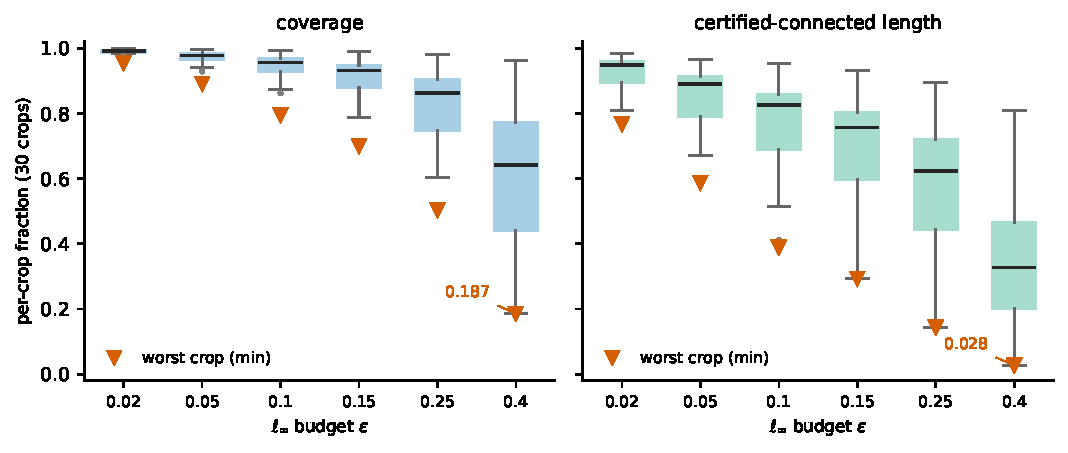
\includegraphics[width=\linewidth]{figs/fig_worstcrop.pdf}
\caption{Per-crop distribution of coverage (left) and certified-connected
length (right) across the 30 real crops at each $\eps$ (box = IQR,
whiskers = range, dots = outliers). The worst crop (min, $\blacktriangledown$)
is marked: the cohort floors are coverage 0.187 and certified connectivity
0.028 at $\eps=0.40$ (each a minimum, on \emph{different} crops), so the
\S\ref{sec:real} headline is a floor over the cohort, not a mean pulled up
by easy crops.}
\label{fig:worstcrop}
\end{figure}

\section{The counterexample constructions}\label{app:constructions}
Figure~\ref{fig:counterexample}'s grids are the regression-test arrays: a
$40\times 40$ field, background score 0.05, ring $8<r<14$ at score 0.95,
interior $r\le 8$ at score 0.5 (fillable case) or 0.05 (unfillable case),
$\eps=0.1$. Under the sandwich: the ring is $\CFG$ in both cases; the
interior is $\POSS$ in the first ($0.5\pm 0.1$ straddles $\tfrac12$) and
$\CBG$ in the second ($0.05+0.1<\tfrac12$). $\beta_1(\CFG)=1$ in both;
only the second survives the all-$\POSS\to$foreground extreme.
Figure~\ref{fig:pinch}'s pinched bar: a $30\times 60$ field, bar rows
13--16, columns 5--54 (inclusive) at 0.95, with the two pinch columns
29--30 at 0.55 --- above threshold (so the skeleton spans) but within
$\eps=0.1$ of $\tfrac12$ (so the two pinch pixels per row are $\POSS$,
and the spanning segment is not certified-connected).

\paragraph{Connectivity is not a diagram functional.} Take three
identical $\CFG$ squares $X, Y, Z$ over $\CBG$ background and one $\CFG$
bridge of fixed shape: joining $X$--$Y$ (map A) or joining $Y$--$Z$ (map
B) produces identical superlevel persistence diagrams in every degree ---
the diagram is location-blind --- yet with designated endpoints in $X$
and $Y$, map A's pair is certified-connected while map B's pair is
certainly separated in every reachable mask. No functional of the
persistence diagram computes the connectivity class; that certificate is
not a persistence statement.

\section{Soundness-check accounting}\label{app:accounting}
Every emitted certified class is checked against 32 reachable masks: the
two deterministic extremes plus 30 random reachable masks. The real-track
total across 30 crops, the four certified classes (components, tessera
cores, corrected cycles, and connectivity segments), and the six-point $\eps$ sweep is
16{,}675{,}936 individual checks --- exactly $32 \times 521{,}123$ class
instances --- with 0 violations. The check for a foreground class asserts
connectivity and presence in the minimal mask; for a background core,
absence from the maximal mask; for a cycle, hole persistence at both
extremes; for a connectivity segment, endpoint connectedness in the
minimal mask.

\paragraph{Random-mask baseline (registered).} To measure \S3.6's
tightness claim, \texttt{random\_baseline.py} plants fillable square rings
(interior area $=c$) and pinched bars (min-cut $c$ verified exactly by
max-flow) and scores the \emph{semantic} violation events --- hole
destroyed, endpoints disconnected --- under two samplers: the uniform
reachable-mask model of \S3.6 and the harness's own (per-mask
$q \sim U(0.1, 0.9)$, iid per pixel). Detection probabilities are computed
exactly (closed form for the ring; full pinch-block enumeration for the
bar) and Monte-Carlo cross-checked; the committed
\texttt{results\_random\_baseline.json} shows fair-coin ring detection
equal to $2^{-c}$ exactly, and the harness sampler decaying exponentially too, but with a
slower base --- $0.9$ rather than $\tfrac12$, times a $1/(c+1)$ factor ---
an advantage of biased sampling that still vanishes as $c$ grows, and every planted violation caught at exactly one
extreme --- rings at $M_{\max}$, bars at $M_{\min}$ --- never the other
(Figure~\ref{fig:missrate}).

\begin{figure}[t]
\centering
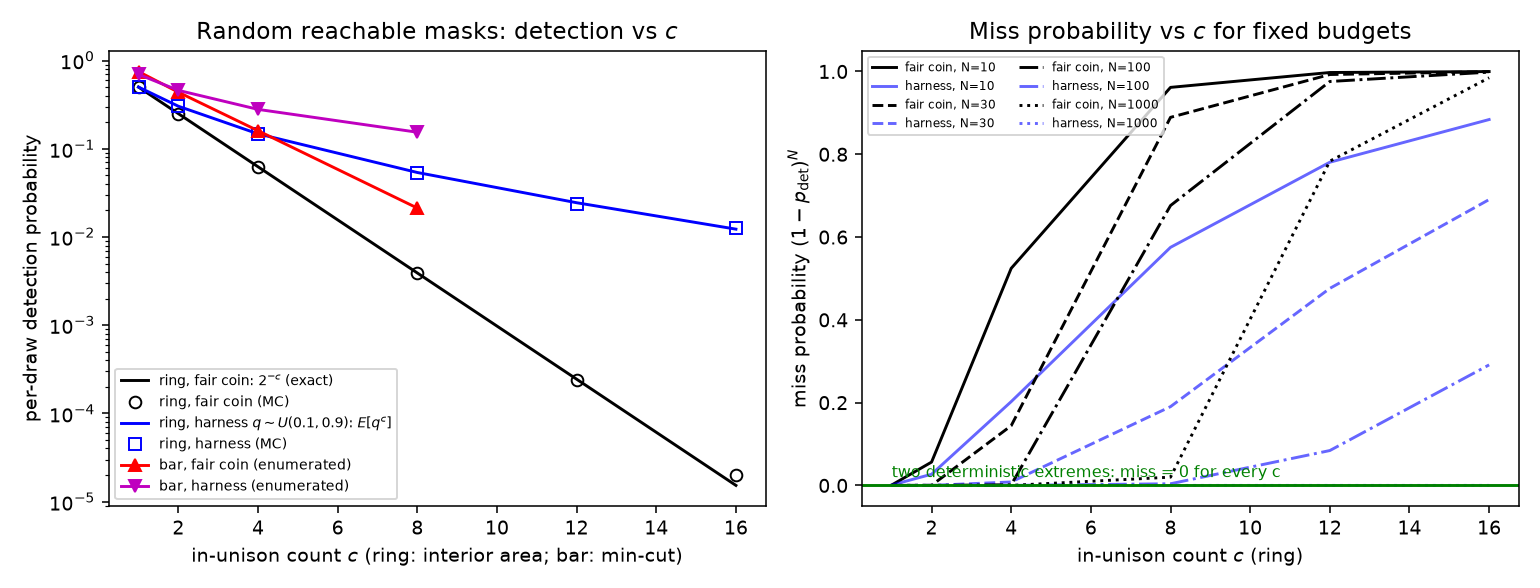
\includegraphics[width=\linewidth]{figs/fig_missrate.png}
\caption{Random-mask baseline (registered). Left: per-draw detection of
planted semantic violations vs the in-unison count $c$; exact laws,
enumeration, and Monte-Carlo agree. Right: miss probability
$(1-p_{\mathrm{det}})^{N}$ at fixed budgets climbs toward one as $c$
grows, while the two deterministic extremes catch every planted violation
with certainty, each at exactly the predicted extreme.}
\label{fig:missrate}
\end{figure}

\section{Related-work delta table}\label{app:delta}
This is the paper's positioning claim in full: for each adjacent method,
\emph{what} it certifies, under \emph{which} threat model, and whether the
guarantee is worst-case, topological, and \emph{checked} rather than
sampled. The bottom row is INTACT, so the table is read as the delta
between this paper and its neighbours. Every cell was verified against the
primary source (staging notes committed in the repo);
\S\ref{sec:related} gives the one-sentence version.

\begin{center}
\small
\setlength{\tabcolsep}{4pt}
\begin{tabular}{L{2.9cm}L{2.7cm}L{2.1cm}L{1.9cm}L{2.05cm}L{2.1cm}}
\toprule
\textbf{Method} & \textbf{Output certified} & \textbf{Threat model} &
\textbf{Worst-case?} & \textbf{Topological?} & \textbf{Checked vs sampled} \\
\midrule
SegCertify \citep{fischer2021segcert} / AdaptiveCertify \citep{anani2024adaptive} &
per-pixel labels & input-space (smoothing) & probabilistic & no & sampled \\
Betti matching \citep{stucki2023betti} + topology-aware losses &
training loss on the learned map & none & no & yes (loss) & n/a (training) \\
Well groups \citep{emp2011wellgroups,bendich2013levelsets} &
level-set homology rank of a fixed field & $\ell_\infty$ on the field &
yes & yes & diagram read; uncomputable in general \citep{franek2015wellgroups} \\
Mandatory critical points \citep{gunther2014mandatory} &
guaranteed critical-point regions & per-vertex interval bounds & yes &
yes & tree pairing / visualization \\
Topology-guaranteed segmentation \citep{topoguarantee2026} &
enforced connectivity/genus of the output & none & no (enforce $\ne$
certify) & yes & optimization \\
Conformal morphological sets \citep{mossina2025conformal} &
statistical coverage of the truth mask & calibration exchangeability &
probabilistic & no & calibrated margin \\
PH-representation robustness \citep{agerberg2025certifying} &
downstream label via persistence features & input Lipschitz & yes
(label) & diagram-metric & Lipschitz bound \\
\midrule
\textbf{INTACT (this paper)} & \textbf{four topological classes of the
segmentation itself} & \textbf{$\ell_\infty$ on $p$} & \textbf{yes} &
\textbf{yes} & \textbf{checked + adversarial harness with witnesses} \\
\bottomrule
\end{tabular}
\end{center}

\section{Compute and runtime}\label{app:compute}
All certification is CPU-only; a single desktop GPU (RTX 4080, 16\,GB) is
used once, for the frozen model's inference over the 30 crops. On one core,
uncontended, the full per-unit cost (certification \emph{plus} the soundness
harness) is ${\approx}51$\,s per mosaic $(\text{crop}, \eps)$ at the 32-mask
setting and ${\approx}104$\,s per retinal $(\text{image}, \eps)$ at 16 masks
(${\approx}36$\,s at 4). Certification proper is only $1$--$14$\,s of that;
the soundness harness --- thousands of certified classes $\times$ the mask
budget --- is the bulk, which is exactly why the two-extreme minimality of
\S\ref{sec:soundness} matters in practice (the extremes are exhaustive, so
the mask budget above two buys only cross-checks). The per-$(\text{unit},
\eps)$ cells are independent, so the whole study is embarrassingly parallel:
the 30-crop mosaic run (\texttt{run\_parallel.py}) and the retinal study
(DRIVE via \texttt{drive\_v2.py} and CHASE's
20-image\,$\times$\,3-normalization\,$\times$\,6-$\eps$ sweep via
\texttt{chase\_parallel.py}) each finish in minutes-to-a-couple-hours of
wall time on the 24-thread machine (64\,GB RAM). A near-linear
implementation of the connectivity segment graph (\S\ref{sec:conn})
was load-bearing: it cut dense-vessel certification from ${>}20$ minutes to
${\approx}14$\,s per $(\text{image}, \eps)$, without which the retinal study
was intractable.

\end{document}
